%%%%%%%%%%%%%%%%%%%%%%%%%%%%%%%%%%%%%%%%%%%%%%%%%%%%%%%%%%%%%%%%%%%%%%%%%%%%%
%
%
%%%%%%%%%%%%%%%%%%%%%%%%%%%%%%%%%%%%%%%%%%%%%%%%%%%%%%%%%%%%%%%%%%%%%%%%%%%%%%

\documentclass[11pt,a4paper]{atlasnote}
\graphicspath{{figures/}}
\usepackage{atlasphysics}
\usepackage{geometry,color,graphicx}
\usepackage{subfigure}
\usepackage{float}
\usepackage{mathrsfs}
\usepackage{rotating}
\usepackage{multirow}
\usepackage{siunitx}
\usepackage{feynmp}
\usepackage{ifpdf}
\ifpdf
\DeclareGraphicsRule{*}{mps}{*}{}
\else
\DeclareGraphicsRule{*}{eps}{*}{}
\fi 

\makeatletter
    \def\endfmffile{%
      \fmfcmd{\p@rcent\space the end.^^J%
      end.^^J%
      endinput;}%
      \if@fmfio
        \immediate\closeout\@outfmf
      \fi
      \ifnum\pdfshellescape=\@ne
        \immediate\write18{mpost \thefmffile}%
      \fi}
    \makeatother



\renewcommand{\topfraction}{0.99}
\renewcommand{\bottomfraction}{0.98}
\renewcommand{\textfraction}{0.0}
\renewcommand{\floatpagefraction}{0.97}

\usepackage{authblk}
\renewcommand\Authands{, } % avoid ``. and'' for last author
\renewcommand\Affilfont{\itshape\small} % affiliation formatting

%%%%%%%%%%%%%%%%%%%%%%%%%%%%%%%%%%%%%%%%%%%%%%%%%%%%%%%%%%%%%%%%%%%%%%%%%%%%%%
% Preamble
%%%%%%%%%%%%%%%%%%%%%%%%%%%%%%%%%%%%%%%%%%%%%%%%%%%%%%%%%%%%%%%%%%%%%%%%%%%%%%

%\title{Cross-section measurement of W boson produced in association with jets}
\title{Searches for the exclusive double diffractive Higgs}
%\author{The ATLAS Collaboration}


\author[a]{L.~Feremenga} %
\author[b]{L.~Nodulman} %
\author[c]{C.~C.~Chau} %
\author[b]{S.~Chekanov} %
\author[a]{J.~Griffiths}%
\author[b]{B.~Blair}%
\author[a]{J.~Yu}%

\affil[a]{University of Texas at Arlington}
\affil[b]{Argonne National Laboratory}
\affil[c]{University of Toronto}

%\clearpage
\draftversion{0.0}

%\clearpage


\abstracttext{ 
The exclusive Higgs could be a clean channel to study Higgs properties. The most popular 
theoretical model for the exclusive Higgs predicts a total cross section of 3 fb at LHC 
8 TeV collision energy. This note 
summarizes a search for the exclusive Higgs boson using ATLAS 8 TeV data, using the 
\hwwll\ decay channel with different flavor leptons in the final state. Selection 
criteria were developed to isolate exclusive processes from inclusive processes. Selection 
criteria that isolate Higgs-like events that were inherited from previous Higgs searches 
were also utilized. A limit of 770 fb on the total cross section of the exclusive Higgs 
production was obtained. 
}

%%%%%%%%%%%%%%%%%%%%%%%%%%%%%%%%%%%%%%%%%%%%%%%%%%%%%%%%%%%%%%%%%%%%%%%%%%%%%%%
% This is where the document really begins
%%%%%%%%%%%%%%%%%%%%%%%%%%%%%%%%%%%%%%%%%%%%%%%%%%%%%%%%%%%%%%%%%%%%%%%%%%%%%%%

% Shorthand for \phantom to use in tables
\newcommand{\pho}{\phantom{0}}
\newcommand{\bslash}{\ensuremath{\backslash}}
\newcommand{\BibTeX}{{\sc Bib\TeX}}
\newcommand{\BHSH}{{\sc BlackHat}-SHERPA}
\newcommand{\HWW}{$H\to WW^{*}\to\ll$}

\begin{document}

\tableofcontents
\clearpage

%%%%%%%%%%%%%%%%%%%%
%\clearpage
\section{Introduction}
\label{sec:introduction}

\par Theoretical studies that attempt to
estimate the event rates for the exclusive diffractive Higgs boson at
the LHC have been previously preformed~\cite{Hdijet}~\cite{canLHC}. 
In these studies rapidity gaps between
the Higgs decay products and the outgoing protons play the most active
role. At high luminosities however, these rapidity gaps are corrupted
by pileup events and can hardly be used to separate exclusive processes from 
inclusive processes. This result has diverted attention to ATLAS' ALFA detectors
which could be used as taggers for the outgoing protons. A search for an
exclusive pion pair has been used to test the feasibility of these ALFA 
detectors~\cite{pionPair}. 
 
\par The most recent experimental searches for exclusive events were done
 at 7 TeV by ATLAS and CMS~\cite{CMSmumu}~\cite{CMSee}~\cite{MonteNote}.
Here isolated lepton pairs from QED production were searched for by looking 
for isolated vertices with only two lepton tracks; no rapidity gaps or 
proton tagging was used. At 8 TeV however the strategy of looking for 
vertices with only two tracks was found to be inefficient using exclusive 
\HWWll\ Monte Carlo samples. Feasibility studies by the tracking group confirmed 
this inefficiency and demonstrated that vertexing algorithms at 8 TeV 
tend to generously associate tracks with vertices. This obviously contaminates the exclusive signal.  

\par In this note a search for exclusive events using an 
algorithm that utilizes neither vertexing, rapidity gaps nor proton tagging is presented. 
Exclusive \HWWll\ events survival rate is improved. 
The note is organized as follows: Section~\ref{sec:theory} 
describes briefly the physics of exclusive diffractive Higgs production.
The Khoze Martin Ryskin (KMR) and CHIDe models are described and their 
sources of theoretical systematic uncertainties are outlined. A discussion of 
the Monte Carlo (MC) sample used to study the signal and a list of backgrounds 
and their MC is outlined as well in this section. Section~\ref{sec:selection} 
describes the object and event selection. Section~\ref{sec:exclusivity} 
introduces the algorithm for selecting exclusive events. Here the signal 
survival rate is quoted and the exclusivity cut is tested in data. Section~\ref{sec:results} 
estimates the expected number of signal events versus background events 
in the signal region.   

%%%%%%%%%%%%%%%%%%%%

%%%%%%%%%%%%%%%%%%%%
\clearpage
\section{Theory}
\label{sec:theory}

\par The Feynman diagram shown in Figure~\ref{fig:exclH} describes the production
of the exclusive double diffractive Higgs boson. In this QCD mechanism two gluons 
interact through a top quark loop to form the Higgs boson
 while a third gluon is exchanged to keep the protons color neutral and hence intact.  
Calculations for this process have been studied extensively. The most popular 
calculations are performed by the KMR and the CHIDe models, which differ very slightly 
and predict similar cross sections~\cite{Khoze}\cite{Cudell}. 
Both models introduce the proton impact factor through the skewed 
unintegrated gluon density~\cite{Martin}, calculate the probability of additional
gluon density using the Sudakov form factor~\cite{Dokshitzer1980269}.
Both models also take into account the probability of soft interaction between the 
outgoing protons. This interaction tends to destroy the intactness of the
outgoing protons, and hence destroys the rapidity gaps associated with 
exclusive processes. There are two main differences between the KMR and the CHIDe models:
 CHIDe uses different limits to compute the Sudakov factor and also includes
an additional K-factor to introduce some NLO corrections. 
As a result, KMR predicts a higher cross section for the exclusive 
double diffractive Higgs than CHIDe. For a 125\GeV\ Higgs KMR predicts
3 fb at $\sqrt{s}=8$\TeV~\cite{Khoze}. 

\begin{figure}[!h]
\centering
\begin{fmffile}{fgraphs}
\begin{fmfgraph*}(200,200)
%bottom and top verticies
  \fmfleft{P1,P2}
  \fmfright{P1',H,P2'}
%incoming protons to gluon vertices
  \fmf{fermion,tension=2,lab=$P_1$}{P1,g1}
  \fmf{fermion,tension=2,lab=$P_2$}{P2,g2}
%blobs at gluon vertices, 0.16w is the size of blob
\fmfblob{.16w}{g1,g2}
\fmf{gluon}{g1,v1}
\fmf{gluon}{g1,g2}
\fmf{gluon}{v2,g2}
%quark loop was here
\fmf{fermion, tension=1, lab.side=left,lab=$t$}{t,v1}
\fmf{fermion, tension=1.2, lab.side=left,lab=$t$}{v1,v2}
\fmf{fermion, tension=1,lab.side=left,lab=$t$}{v2,t}
\fmf{dashes, lab=$H$}{t,H}
%%gluon from P1 to loop
%\fmf{gluon}{g1,K1}
%%gluon from P2 to loop
%\fmf{gluon}{g2,K2}
%%quark loop was here
%\fmf{fermion, lab.side=right,lab=$b$}{K3,H}
%outgoing protons
\fmf{fermion}{g1,P1'}
\fmf{fermion}{g2,P2'}
%freeze everything in place
%\fmffreeze
%\renewcommand{\P}[3]{\fmfi{plain}{%
%    vpath(__#1,__#2) shifted (thick*(#3))}}
%%lines on P1
%\P{P1}{g1}{2,-1}
%\P{P1}{g1}{-2,1}
%%lines on p2
%\P{P2}{g2}{2,1}
%\P{P2}{g2}{-2,-1}
%%lines on P1'
%\P{g1}{P1'}{-2,-1}
%\P{g1}{P1'}{2,1}
%%lines on P2'
%\P{g2}{P2'}{-2,-1}
%\P{g2}{P2'}{2,1}
\end{fmfgraph*}
\end{fmffile}
\caption{}
\label{fig:exclH}
\end{figure}

\par There are two main sources of theoretical systematic uncertainties
that have to be studied: upper and lower Sudakov form factor scales, unintegrated
gluon densities. Uncertainties associated with the 
rapidity gap survival probability were originally studied for the 
Tevatron and subsequently for the LHC~\cite{Khoze2000wk}. 
In this analysis we will not use rapidity gaps for event selection so 
uncertainties from rapidity gaps are estimated to be minimal. 

\subsection{Signal and Background Models}
\par Both the KMR and CHIDe models are implemented in the Forward Physics Monte Carlo (FPMC).
For signal we generate exclusive \hwwll\ within KMR using FPMC 
and shower with Herwig. The results are then run through the full simulation
of the ATLAS detector. This signal is characterized by very little activity 
around the dileptons. 
\par Background processes can be separated into exclusive and inclusive. 
Inclusive backgrounds are those in which the two protons dissociate and 
the by-products are detected by the ATLAS detector. All these backgrounds 
are estimated using several MC samples except the W+jets background, in 
which the jet is misidentified as a lepton. A 
tested and verified data-driven method is used to estimate W+jets. See 
Section VIC from Ref.~\cite{ATLASCONF2014060} for a detailed description 
of this method. The rest of the backgrounds are listed in Table~\ref{table:background}.

\par The Z/$\gam^*$+jets background is dominated by \zGamtau+jets in 
which the taus decay leptonically to a different flavor
channel. If the jets are misidentified as \MET\ the two leptons from the final state 
would fake the \hwwll\ signature. Of the \zGamtau+jets processes, the 0-jet process
contributes the most signal contamination because it has the least activity
around the dilepton system. These processes are generated with Alpgen and showered with Herwig. 

\par \ttbar\ is a background to the Higgs signature when the two top quarks decay to a WW system
and a pair of b jets. MC@NLO is used to generate this process and Jimmy is used for showering. 
A single top quark is also a background process because a b jet can be misidentified 
as a lepton. Powheg is used to generate single top events and the showering is done 
with Pythia. 

\par Because the signal is produced through gluon exchanges (See  Figure~\ref{fig:exclH}), ggF Higgs
is a background. ggF Higgs is generated with Powheg and showered with Pythia8. Apart from the intensity 
of activity about the dilepton system, the kinematics of ggF Higgs is identical to that of 
the exclusive Higgs.

\par Another irreducible inclusive background is a pair of W bosons. It is refered to as 
{\it inclusive WW} in this note. The final decay products are identical to signal so 
kinematic distributions are used to separate this background from signal. This is modelled 
by Powheg and Pythia.

\par The rest of the inclusive backgrounds will be referred in this note as {\it Other VV}. This is because they
all constitute a pair of vector bosons. These are $W\gamma$, $W\gamma^*$, $Z\gamma$, $Z\gamma^*$, ZZ, WZ and 
double-parton interaction (DPI). The MC samples for these processes are listed in Table~\ref{table:background}. 
     
\par The main contribution to the exclusive background is the exclusive boson pair. 
Exclusive lepton pairs have a very small cross section compared to exclusive boson pairs. Regardless, 
they are also considered in this study. 
In both cases photons are exchanged, in contrast to gluons exchanged 
in the exclusive Higgs production.
Three diagrams contribute to the exclusive boson pairs. Figure~\ref{fig:excWW} shows the three different diagrams.
In a purely elastic process none of the two protons dissociate during the collision. The intact protons 
vanish along the beamline and the fiducial region sees only the WW decay products. In a Single Dissociative (SD) process
one of the protons dissociate, but the remnants of the dissociation 
vanish along the beamline. A Double Dissociative (DD) process is similar to an inclusive process, but the proton remnants disappear along the beamline.
The three processes have identical kinematic process, so it is impossible to 
distinguish them. Only the purely elastic diagram is modeled by the available MC, Herwig++. 
Data driven methods are used to estimate the SD and DD contributions.    

\begin{figure}[!htb]
\minipage{0.32\textwidth}
\begin{fmffile}{fgraphs0D}
\begin{fmfgraph*}(80,60)
\fmfleft{i1,i2}
\fmfright{o1,o2,o3,o4}
\fmf{fermion}{i1,v1}
\fmf{fermion}{v1,o1}
\fmfv{}{o1}
\fmf{fermion}{i2,v2}
\fmf{fermion}{v2,o4}
\fmfv{}{o4}
\fmf{photon,label=$\gamma$}{v1,v3}
\fmf{photon}{v3,o3}
\fmfv{label=$W^+$}{o3}
\fmf{photon,label=$\gamma$}{v2,v3}
\fmf{photon}{v3,o2}
\fmfv{label=$W^-$}{o2}
\fmfdot{v3}
\end{fmfgraph*}
\end{fmffile}
\endminipage\hfill
\minipage{0.32\textwidth}
\begin{fmffile}{fgraphsSD}
\begin{fmfgraph*}(80,60)
\fmfleft{i1,i2}
\fmfright{o1,o2,o3,o4,o5,o6}
\fmf{fermion}{i1,v1}
\fmf{fermion}{v1,o1}
\fmfv{}{o1}
\fmf{fermion}{i2,v2}
\fmfforce{.5w,.8h}{v2}
\fmf{dashes_arrow}{v2,o4}
\fmfv{}{o4}
\fmf{photon,label=$\gamma$}{v1,v3}
\fmf{photon}{v3,o3}
\fmfv{label=$W^+$}{o3}
\fmfforce{w,0.65h}{o3}
\fmf{photon,label=$\gamma$}{v2,v3}
\fmf{photon}{v3,o2}
\fmfv{label=$W^-$}{o2}
\fmfforce{w,0.35h}{o2}
\fmf{dashes_arrow}{v2,o6}
\fmf{dashes_arrow}{v2,o5}
\fmfforce{w,h}{o6}
\fmfforce{w,0.9h}{o5}
\fmfforce{w,0.8h}{o4}
\fmfdot{v3}
\end{fmfgraph*}
\end{fmffile}
\endminipage\hfill
\minipage{0.32\textwidth}%
\begin{fmffile}{fgraphsDD}
\begin{fmfgraph*}(80,60)
\fmfleft{i1,i2}
\fmfright{o1,o2,o3,o4,o5,o6,o7,o8}
\fmf{fermion}{i1,v1}
\fmf{dashes_arrow}{v1,o1}
\fmf{dashes_arrow}{v1,o2}
\fmf{dashes_arrow}{v1,o3}
\fmfforce{.5w,0.15h}{v1}
\fmfforce{w,0}{o1}
\fmfforce{w,0.05h}{o1}
\fmfforce{w,0.1h}{o2}
\fmfforce{w,0.15h}{o3}
\fmf{photon,label=$\gamma$}{v1,v3}
\fmf{photon}{v3,o5}
\fmfv{label=$W^+$}{o5}
\fmfforce{w,0.7h}{o5}
\fmf{fermion}{i2,v2}
\fmfforce{.5w,0.85h}{v2}
\fmf{photon,label=$\gamma$}{v2,v3}
\fmf{photon}{v3,o4}
\fmfv{label=$W^-$}{o4}
\fmfforce{w,0.3h}{o4}
\fmf{dashes_arrow}{v2,o8}
\fmf{dashes_arrow}{v2,o7}
\fmf{dashes_arrow}{v2,o6}
\fmfforce{w,h}{o8}
\fmfforce{w,0.95h}{o7}
\fmfforce{w,0.9h}{o6}
\fmfdot{v3}
\end{fmfgraph*}
\end{fmffile}
\endminipage
\caption{Diagrams that contribute to the exclusive WW processes. [Left] 
A purely elastice process. No proton dissociates and the two protons vanish along the beamline. [Middle]
A single dissociative (SD) process. One proton dissociates but vanishes along the beamline. [Right]
A double dissociative (DD) process. Both protons dissociate but the remnants vanish along the beamline.
Rapidity gaps are present in all three diagrams and the kinematic distributions are identical, so
they are indistinguishable.}
\label{fig:exclWW}
\end{figure}

\begin{table}[!h]
\begin{center}
\begin{tabular}{l|l}
Inclusive Background & Exclusive Background \\
\hline
Drell Yan Z/$\gamma^*$+jets (Alpgen+Herwig) & 															  WW (Herwig++) \\
W$\gamma$ +jets (Alpgen+Jimmy) & $l^{+}l^{-}$ (Herwig++)\\
WZ, WW, ZZ, ggF Higgs (Powheg+Pythia8) 														& \\
\ttbar\ (MC@NLO+Jimmy) & \\
single top (AcerMC+Pythia) & \\
Z$\gamma$ +jets (Sherpa) & \\
\end{tabular}
\caption{Background samples used.}
\label{table:background}
\end{center}
\end{table}

\subsection{Data Samples}
All the data used is from the ATLAS 2012 8~\TeV\ run and sums up to 
a total integrated luminosity of 20.3~\ifb. The D3PDs used are the most up-to-date and are 
identified with the tag p1328/p1329. The integrated luminosity is obtained 
through an ATLAS luminosity calculator~\cite{lumi}. 

%%%%%%%%%%%%%%%%%%%%

%%%%%%%%%%%%%%%%%%%%
\clearpage
\section{Event and Object Selection}
\label{sec:selection}

\par At preselection, events must pass an OR of 
\verb% EF_e24vhi_medium1%, \verb% EF_mu24i_tight%,\\
\verb% EF_e60_medium1%, \verb% EF_mu36_tight%, 
\verb% EF_e12Tvh_medium1_mu8%, 
 \verb% EF_mu18_tight_mu8_EFFS% and \verb% EF_2e12Tvh_loose1%
 to get considered for analysis. They must also have exactly two leptons 
with $\pt>15$~\GeV. A reconstructed primary vertex is not required to have 
a minimum number of tracks associated with it.  
All other preselection cuts are identical to those used for the 
\HWW\ study in Ref.~\cite{ATLASCONF2014060}. 

\par The electron identification criteria closely follows the 
 standard \HWW\ selection which relies on a likelihood-based method to
identify electrons from electromagnetic (EM) showers and Inner Detector (ID) tracks. 
A more detailed description of this method can be found in Ref. ~\cite{ATLASCONF2014060}.
EM showers and ID tracks are required to have $\pt > 15$~\GeV and lie in 
pseudorapidity less than 2.47 and out of the detector crack 
( [1.37,1.52]). Electron candidates with $15<\pt<25$~\GeV have to satisfy the very tight 
likelihood requirement and those with $\pt>25$~\GeV have to satisfy the medium 
likelihood requirement. This is because the latter are less likely to be misidentified 
objects. Calorimeter isolation is also imposed on electron 
objects by considering the energy deposited in a cone of $\Delta R = 0.3$ 
around the electron object cluster. Track isolation is also considered by taking 
the sum \pt\ of all the tracks with $\pt>400$~\MeV\ within a cone 
of size $\Delta R = 0.3$. To separate these electron objects from prompt 
electrons, impact parameter variables are used. The transverse impact parameter $d_0$
is required to satisfy $|d_0|/\sigma_{d_0}<3.0$ where $\sigma_{d_0}$ is the uncertainty on 
$d_{0}$. The longitudinal impact parameter must satisy $|z_0\sin\theta|<0.04$ mm. This improves 
the probability of selecting leptons that originate from the primary vertex. Figure~\ref{fig:electrons}
shows the \pt\ and $\eta$ distributions for electrons that pass all these requirements.   

\begin{figure}[!h]
\centering
\begin{tabular}{c}
	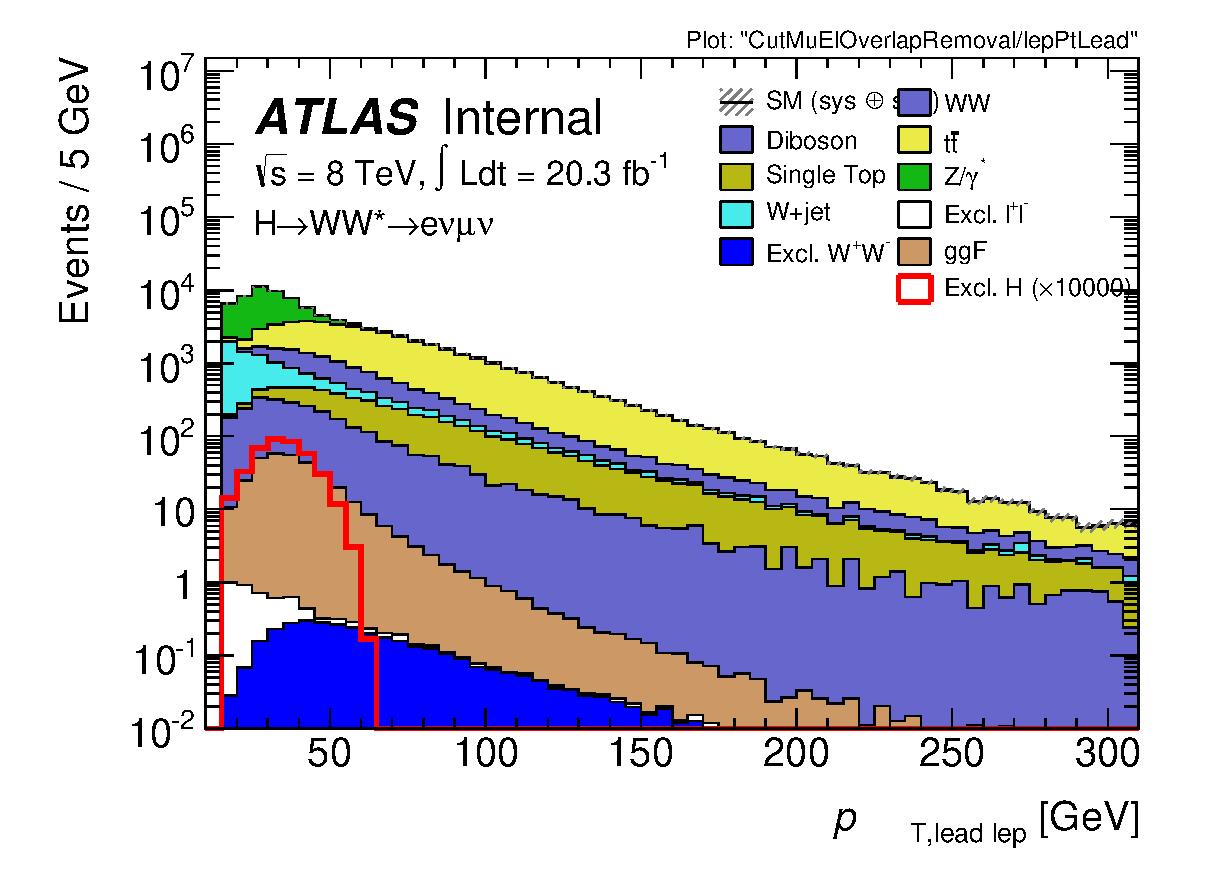
\includegraphics[width=0.5\linewidth]{em_CutMuElOverlapRemoval_lepPtLead_mh125_log.eps}
	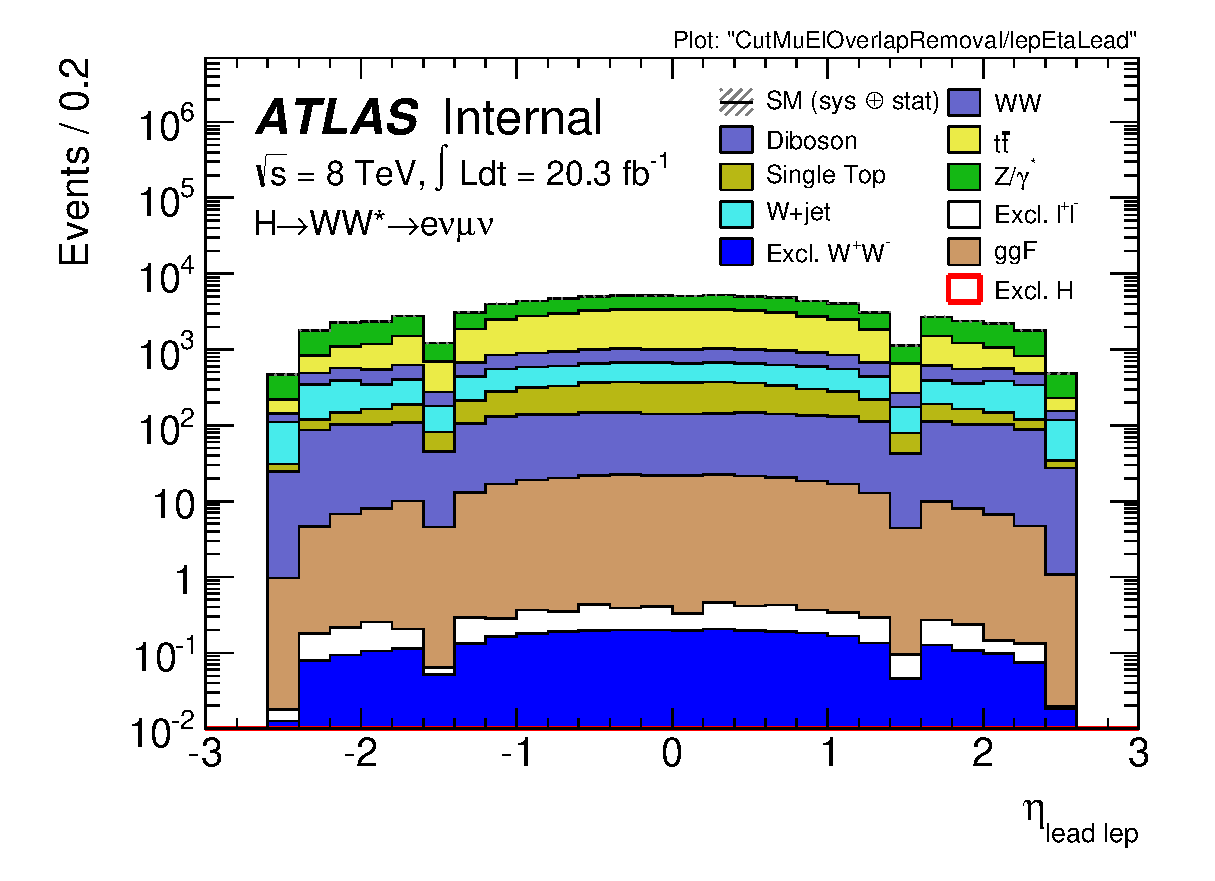
\includegraphics[width=0.5\linewidth]{em_CutMuElOverlapRemoval_lepEtaLead_mh125_log.eps}\\
\end{tabular}
\caption{\pt\ [left] and $\eta$ [right] distributions for electron candidates that pass 
all the electron selection criteria. }
\label{fig:electrons}
\end{figure}
%
\par Candidates for muon objects should be objects with matched hits from the ID and the 
Muon Spectrometer (MS). The algorithms that match ID tracks to MS tracks are described 
in detail in Ref.~\cite{Aad2014rra}. These objects are further required to have 
$\pt > 15$~\GeV\ and must lie within pseudorapidity of 2.47. Muon selection is insensitive 
to the calorimeter crack that covers $1.37<|\eta|<1.52$. That is the reason why the only $\eta$
requirement imposed on muon candidates is for them to lie within 2.47 in $\eta$.
The sum of the pixel hits and dead sensors should be at least 1.
The sum of sct hits and dead sensors should also be at least 5.  This ensures that the 
ID track is a good candidate for matching with an MS track. Track isolation criteria is 
identical to that imposed on electron candidates. No calorimeter isolation is required 
on muons. Figure~\ref{fig:muons} shows the \pt\ and $\eta$ distribution of muon candidates 
that pass all the muon selection criteria.

\begin{figure}[!h]
\centering
\begin{tabular}{c}
	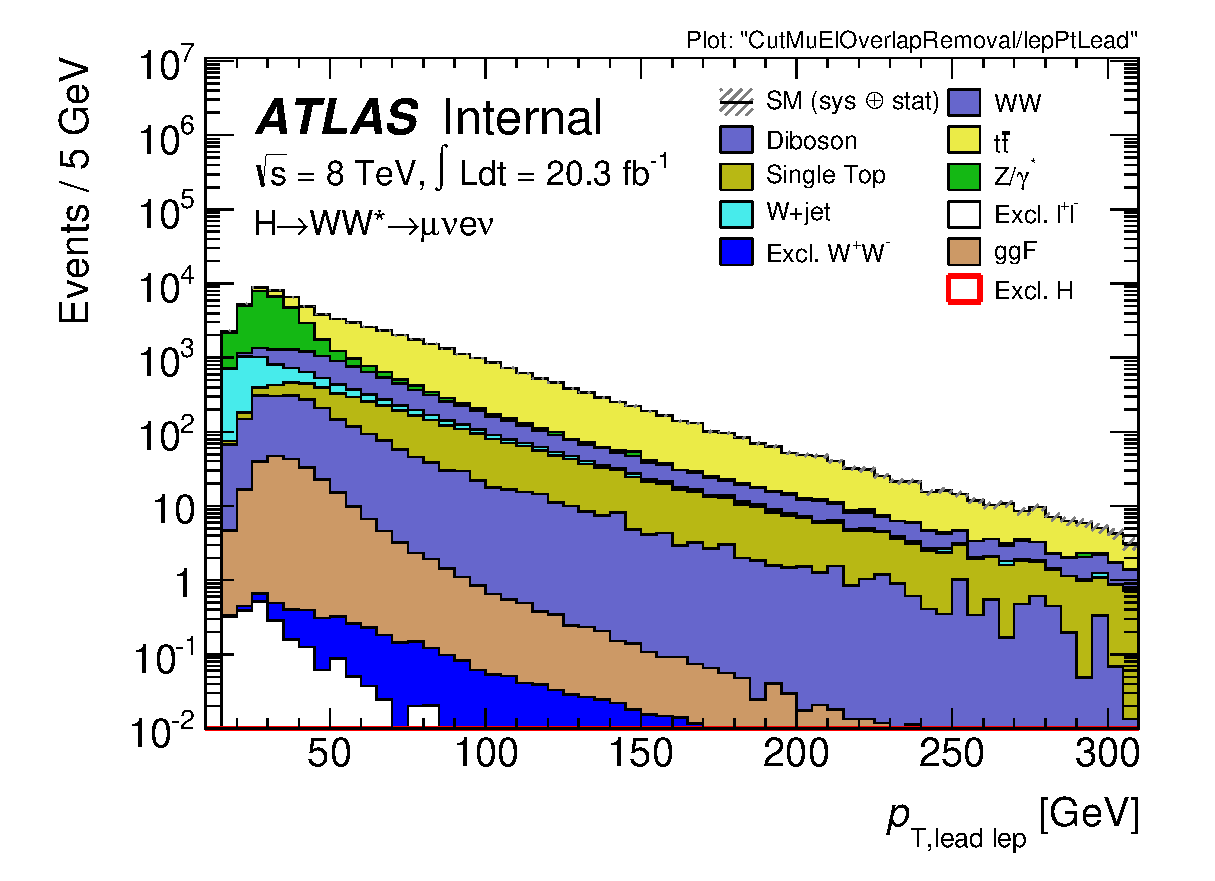
\includegraphics[width=0.5\linewidth]{me_CutMuElOverlapRemoval_lepPtLead_mh125_log.eps}
	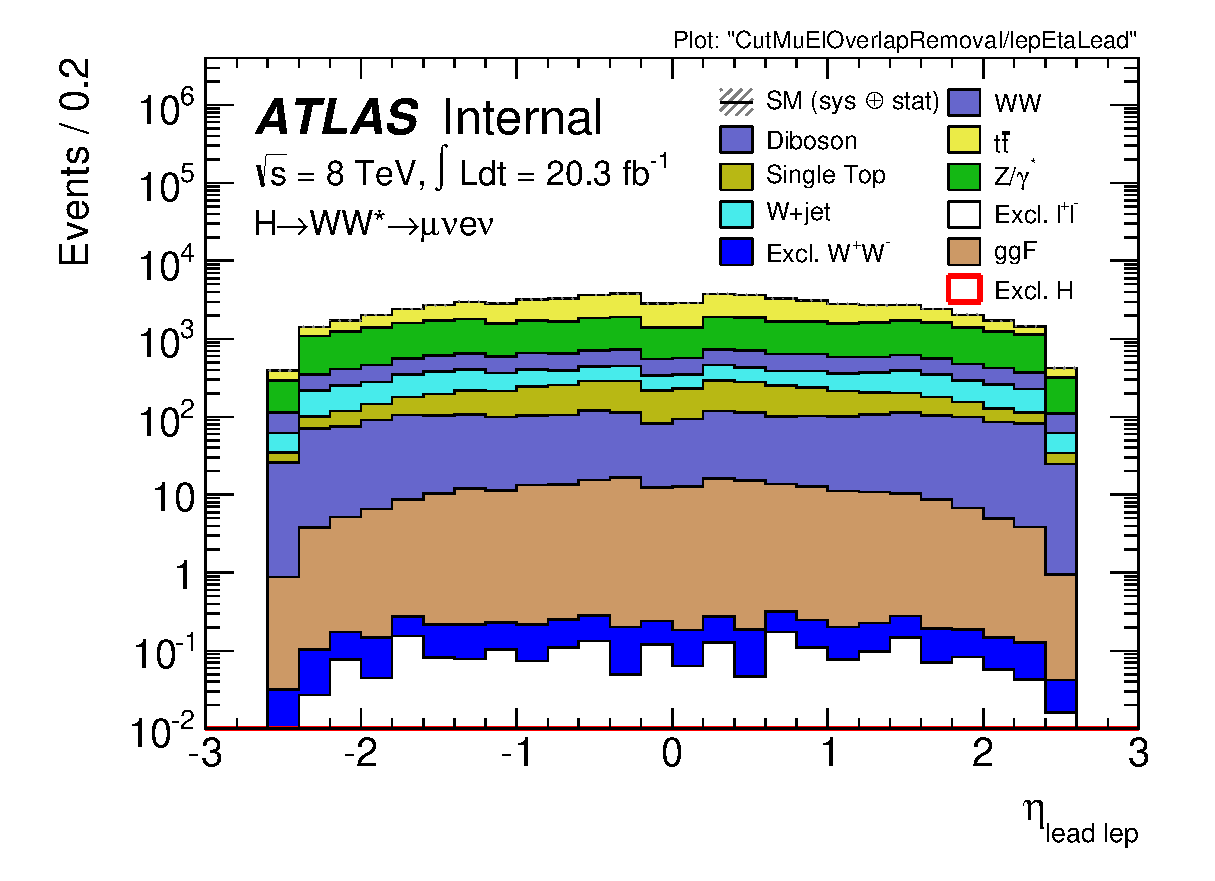
\includegraphics[width=0.5\linewidth]{me_CutMuElOverlapRemoval_lepEtaLead_mh125_log.eps}\\
\end{tabular}
\caption{\pt\ [left] and $\eta$ [right] distributions for muon candidates that pass all the 
muon selection criteria.}
\label{fig:muons}
\end{figure}

\par Electrons and muons can sometimes be very close in $\eta-\phi$ space. If an electron and 
a muon are within $\Delta R<0.1$, where $\Delta R = \sqrt{\eta^2 + \phi^2}$, the electron is removed and
the muon is kept. This is motivated by the theory that the muon would have undergone 
bremsstrahlung. If an electron track is seen in the muon spectrometer, it is removed. If two electrons are 
within $\Delta R<0.1$, the electron with higher \et\ is kept and the other one is discarded. We will 
refer to this process as {\it Electron-Muon Removal} in this note. 

\par Tracks are required to have at least 1 pixel hit and at least 4 sct hits. The minimum \pt\ 
that achieved on these tracks is 400 MeV. Availability of low-\pt\ tracks increases rejection on
QCD multijets and improves the signal survival efficiency. Reasons for this assertion will become 
clearer after the exclusivity selection criteria is discussed in detail in section~\ref{sec:exclusivity}.  
 Track candidates are also required to be within $|\eta|<2.47$. This is in line with the lepton angular 
selection criteria. Figure~\ref{fig:nTracks} shows the number of tracks that pass this criteria. 

\begin{figure}[!h]
\centering
	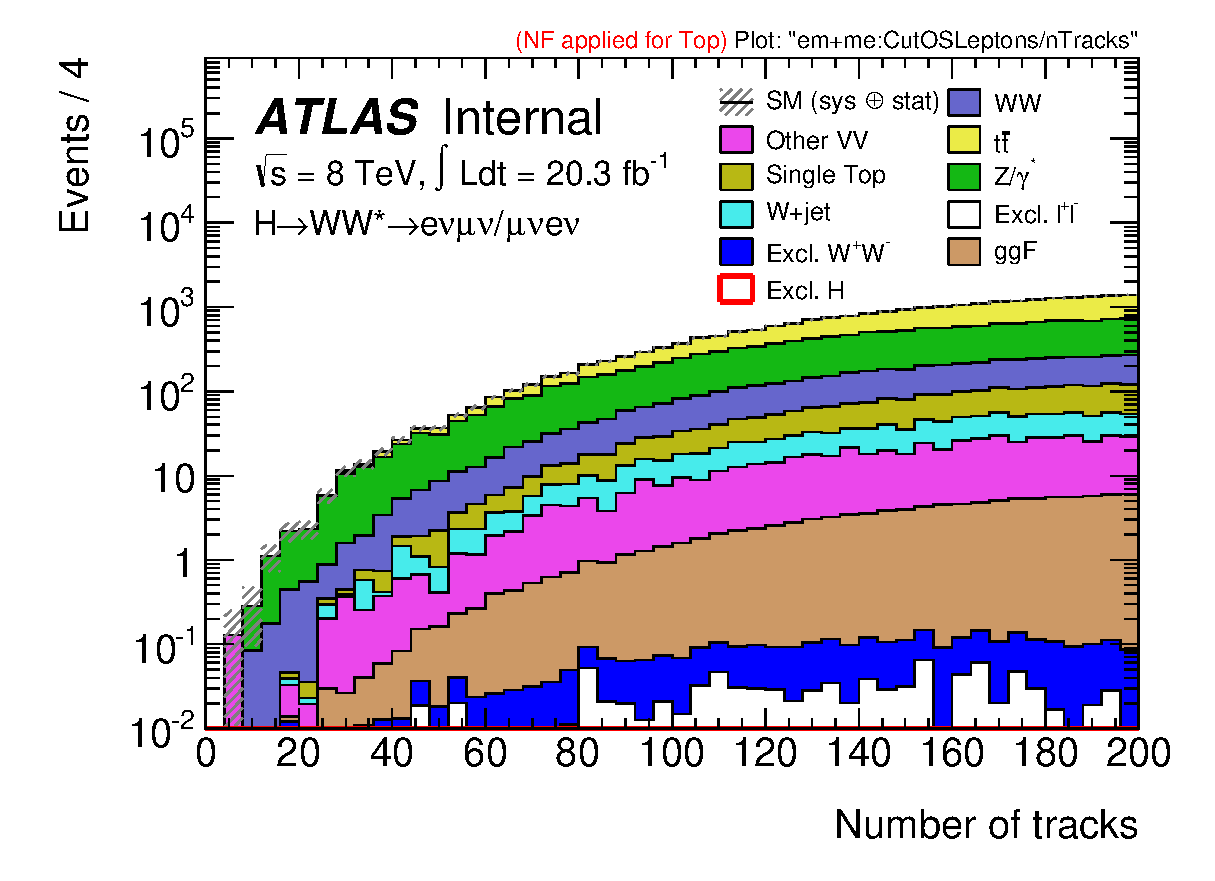
\includegraphics[width=0.5\linewidth]{emme_CutOSLeptons_nTracks_mh125_log.eps}\\
\caption{Number of track candidates that pass the track selection criteria.}
\label{fig:nTracks}
\end{figure}

\par The signal region for events that pass the pre-selection criteria is carefully 
designed to select events that have Higgs-like kinematic properties. 
An exclusivity requirement is further imposed on these events to select events with additional exclusivity-like kinematic properties.
The lepton with higher \pt\ (of the two selected leptons) is required to have $\pt>25$ GeV. This will be refered to as the 'leading 
lepton'. The second lepton, with lower \pt\ is required to have $\pt>15$ GeV. It will 
be refered to as the 'sub-leading lepton'. The high \pt\ selection on the leptons  is 
meant to reduce W+jets and QCD multi-jets backgrounds, where low-\pt\ jets are 
mis-identified as leptons. To exploit the fact that the SM Higgs is neutral, the 
leading and sub-leading leptons are required to be of opposite sign. This cut will be refered to 
as 'OS Leptons' in this note. 
\par The invariant mass of the dilepton system \mll, is demanded to 
be fall within 10 GeV and 55 GeV. The reason for a lower bound is that 
some of the backgrounds such at Z+jets are not modelled correctly at low \mll. In this analysis
only Z+jets MC samples generated at $\mll>10$ GeV are used. Figure~\ref{fig:mllOSleptons}
shows the \mll\ distribution for events that pass the preselection cuts, lepton \pt\ cuts
and the opposite sign requirement on the leptons. The $\mll>10$ GeV cut yields a 
signal survival efficiency of 98\%. Figure~\ref{fig:mllOSleptons} also justifies an upper bound on 
\mll\ for Higgs events. Since the Higgs boson is of spin zero, \mll\ tends to peak at lower
 values than for the WW backgrounds. A $\mll<55$ GeV cut rejects 75\% of inclusive WW background 
and keeps 86\% of signal. 

\begin{figure}[!h]
\centering
	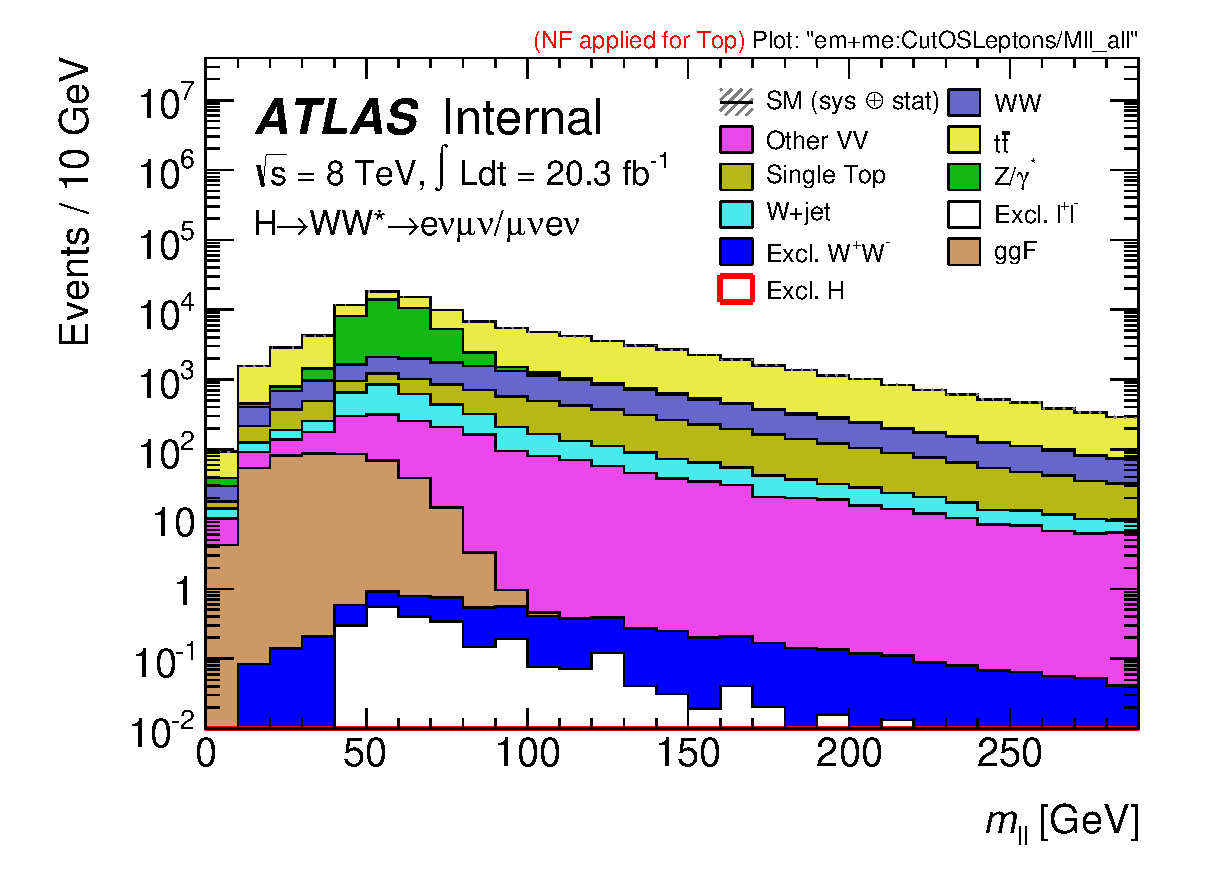
\includegraphics[width=0.5\linewidth]{emme_CutOSLeptons_Mll_all_mh125_log.eps}\\
\caption{\mll\ distribution for signal (scaled by $10^4$) and relevant backgrounds for 
events that pass preselection, lepton \pt, and OS lepton cuts. Z+jets are not well modelled 
for $\mll<10$ GeV, so we consider events with $\mll>10$ GeV. Signal survival after this cut 
is 98\%. An $\mll<55$ GeV cut further rejects 75\% of WW background while keeping 86\% of signal.}
\label{fig:mllOSleptons}
\end{figure}

\par The neutrinos in the signal final state are identified by a momentum imbalance in the detector.
This imbalance is quantified by the variable 'missing transverse momentum',
\met\ that is calculated as 

\begin{equation}
\met = - \left (\sum_{selected}\pt + \sum_{soft}\pt \right )
\end{equation}   

where $\sum_{selected}\pt$ is the vectorial sum of \pt\ from 
all the objects identified by ATLAS identification 
algorithms, such as leptons, photons and jets. In this analysis these 
objects are required to have $\pt>20$ GeV. $\sum_{selected}\pt$ is the vectorial sum 
of \pt\ from all other objects that have low values of \pt, extracted 
from tracks with $\pt>0.5$ GeV that originate from the primary vertex. 
Both \met and its relative direction to leptons and jets are effective variables 
in rejecting Drell-Yan \tautau\ background, where \met\ 
aligns with a final state lepton. A special variable, \metRel (see Ref.~\cite{ATLASCONF2014060} for 
a more detailed description of this variable) is used to quantify how close in the transverse 
plane \met\ is to leptons and jets:

\begin{equation}
\metRel = \begin{cases}
				 \met\sin\Delta\phi_{near} & \text{if $\Delta\phi_{near}<\pi/2$} \\
				 \met & \text{otherwise,}
					\end{cases}
\end{equation}  

where $\Delta\phi_{near}$ is the azimuthal separation of \met\ and the nearest 
high-\pt jet or lepton. Figure~\ref{met} shows \met\ [left] and \metRel\ [right] for events that pass the 
pre-selection, electron-muon removal cuts, lepton \pt\ cuts, the 10 GeV \mll minimum requirement and the opposite sign requirement
on the leptons. For events with 0 or 1 jets, we demand $\met>20$ GeV. For events with 
2 or more jets, we demand  $\metRel>25$ GeV. These criteria are discussed in detail, with 
supporting \met\ and \metRel\ distributions, in Ref.~\cite{ATLASCONF2014060}. As a result Drell-Yan \tautau\ 
and backgrounds with a misidentified lepton are reduced. 

\begin{figure}[!h]
\centering
\begin{tabular}{c}
	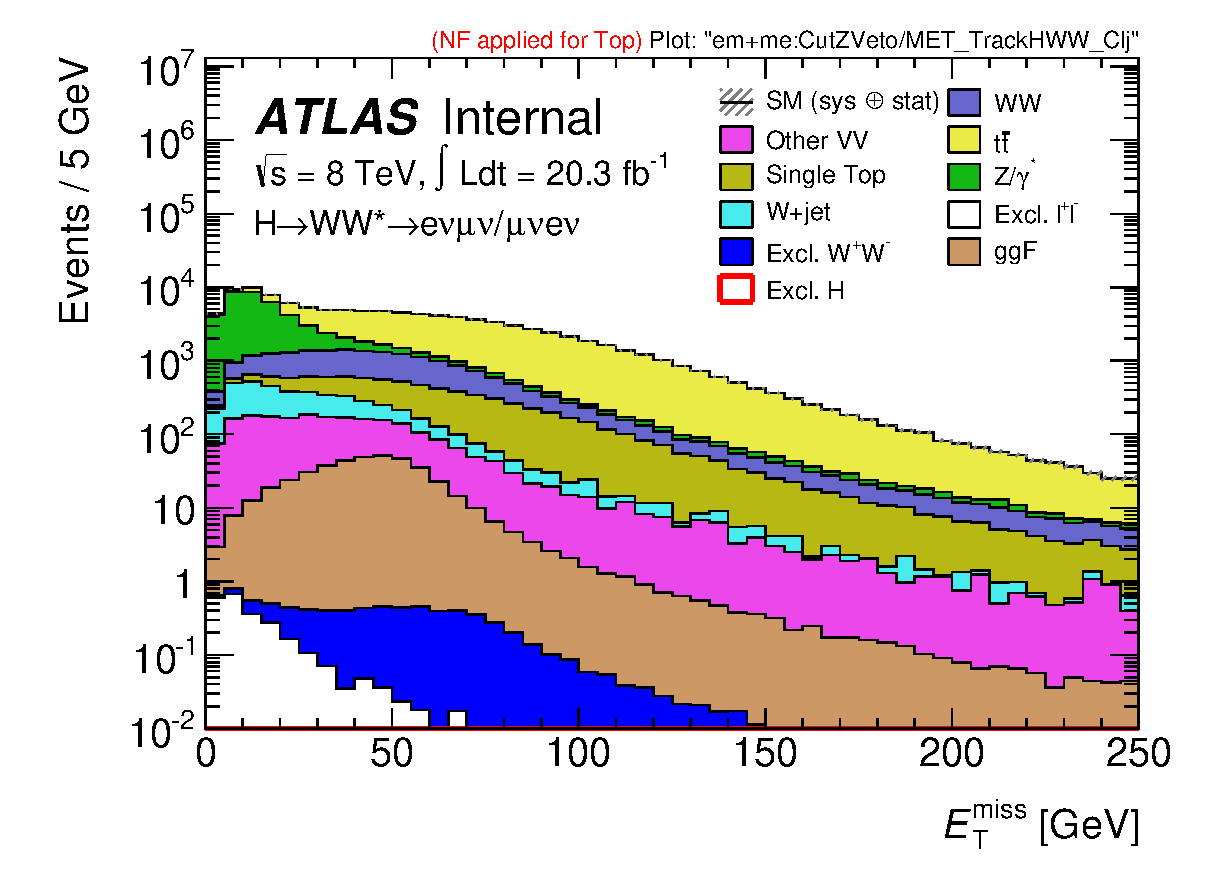
\includegraphics[width=0.5\linewidth]{emme_CutZVeto_MET_TrackHWW_Clj_mh125_log.eps}
	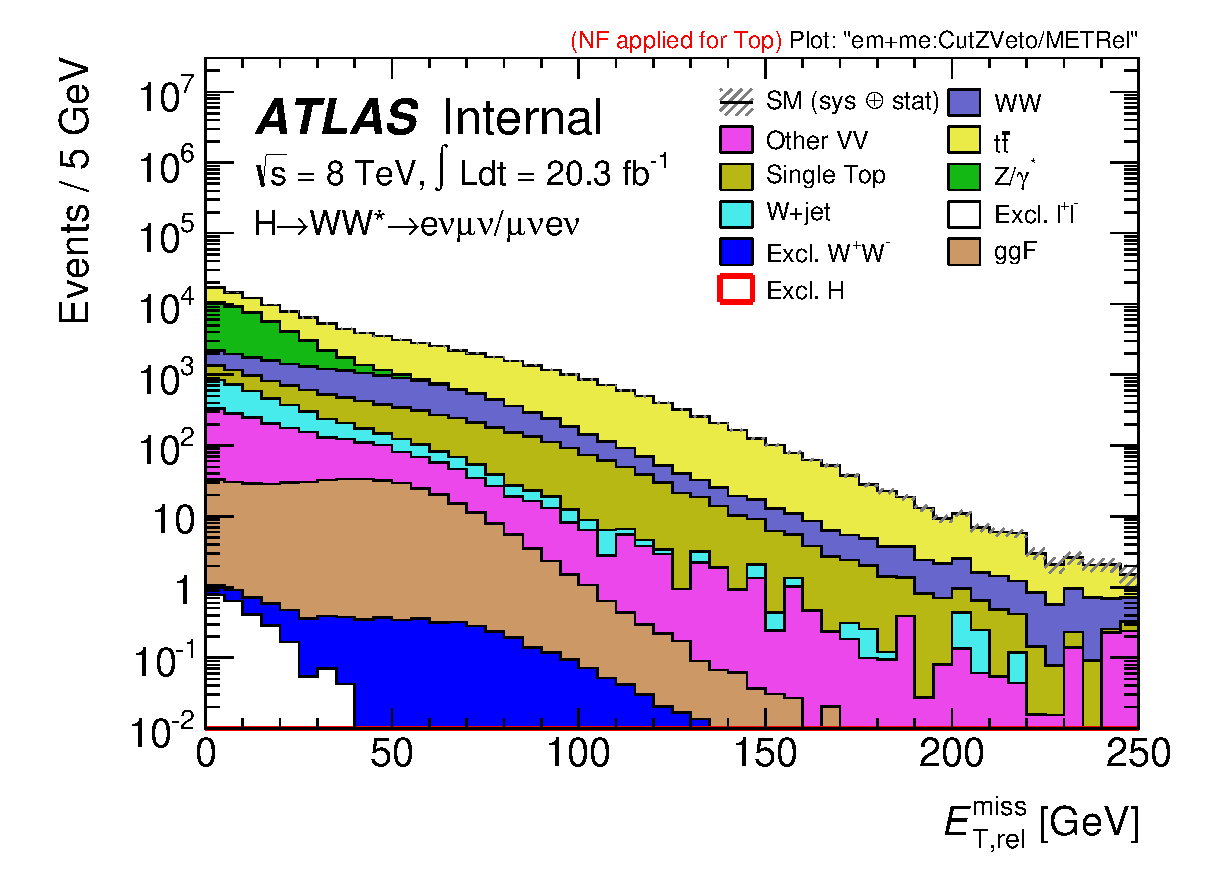
\includegraphics[width=0.5\linewidth]{emme_CutZVeto_METRel_mh125_log.eps}\\
\end{tabular}
\caption{\met\ [left] and \metRel\ [right] for events that pass pre-selection, electron-muon removal, lepton \pt,
$\mll>10$ GeV cut and the opposite sign requirement on the leptons. These variables are crucial in reducing 
Drell-Yan \tautau\ and those backgrounds that have a misidentified lepton.}
\label{fig:met}
\end{figure}

\par To ensure that \met\ is not mismeasured, it is important to establish some separation in $\phi$ 
between \met\ and the dilepton system. The variable \dphillmet\ shown in Figure~\ref{fig:dphillmet}
quantifies this separation. We demand $\dphillmet>\pi/2$ for the signal region. As shown in Figure~\ref{fig:dphillmet} 
this requirement suppresses W+jets and Drell-Yan \tautau. \ptll\ is also used in this analysis to suppress
\tautau\ Drell-Yan backgrounds. The right plot in Figure~\ref{fig:dphillmet} shows that $Z/\gamma^*\to\tautau$ tends to 
have low \pt. In this analysis we demand $\ptll>30$ GeV and keep 90\% of signal. 

\begin{figure}[!h]
\centering
\begin{tabular}{c}
	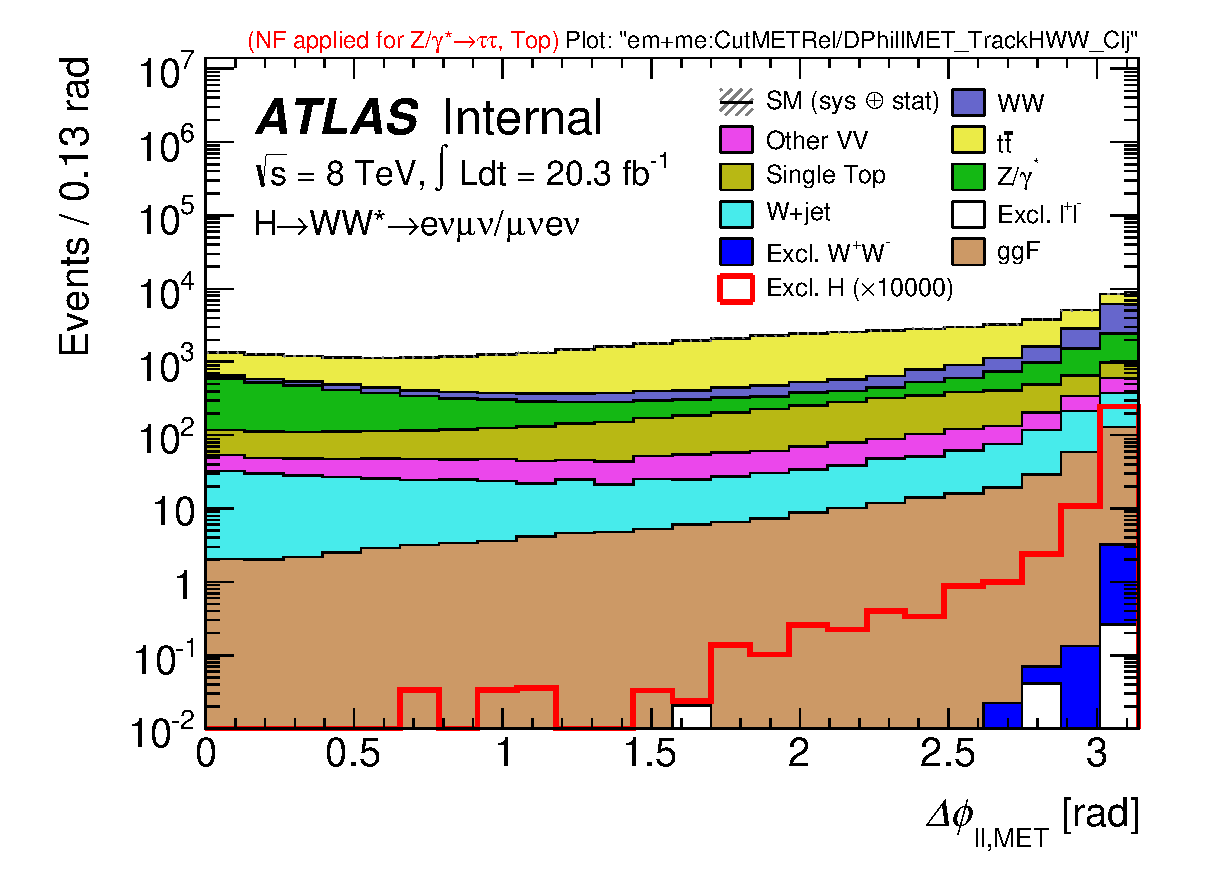
\includegraphics[width=0.5\linewidth]{emme_CutMETRel_DPhillMET_TrackHWW_Clj_mh125_log.eps}
	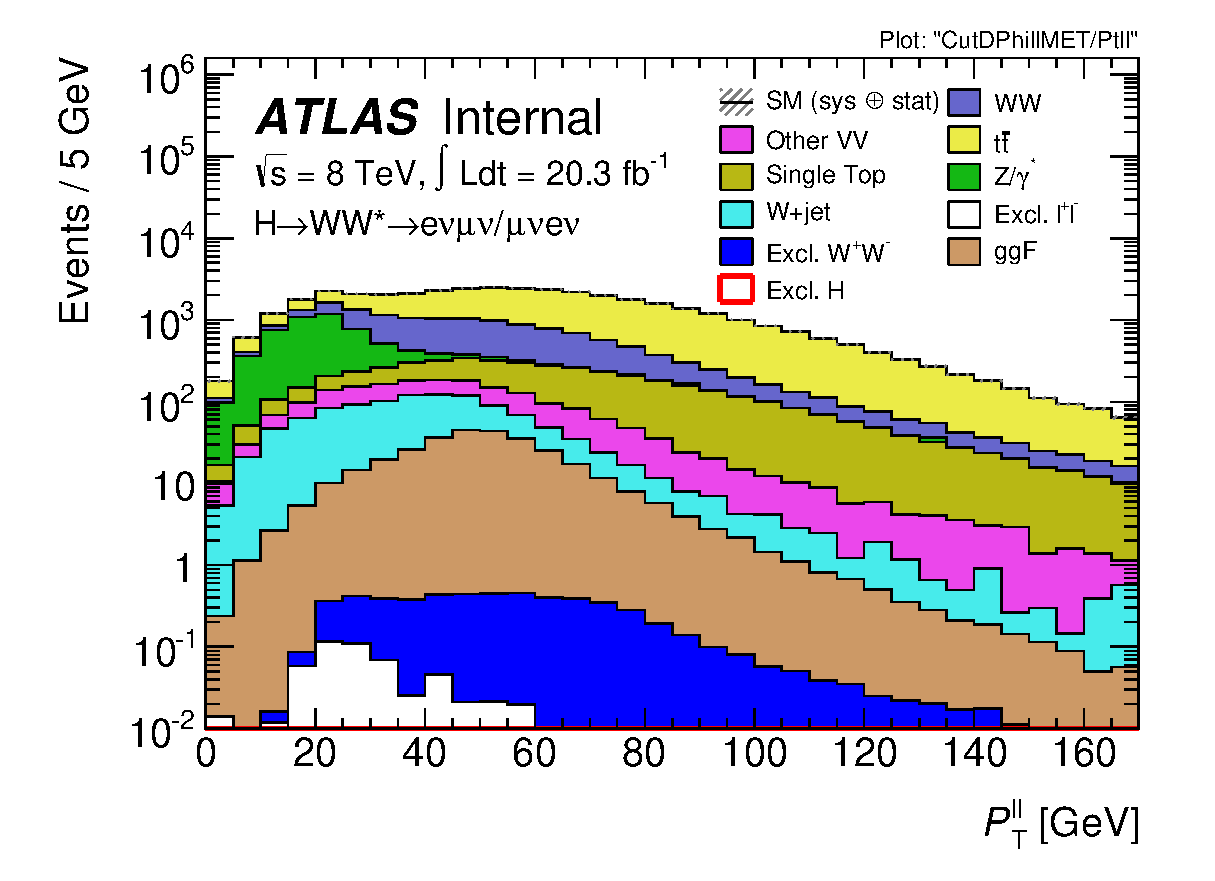
\includegraphics[width=0.5\linewidth]{emme_CutDPhillMET_Ptll_mh125_log.eps}\\
\end{tabular}
\caption{\dphillmet\ [left] quantifies separation in $\phi$-space between \met\ and the dilepton system. This 
is important to suppress mismeasurement of \met\ and further suppresses W+jets and Drell-Yan \tautau\ backgrounds.
\ptll\ [right] is also a good variable for suppressing Drell-Yan \tautau. Signal region demands $\ptll>30$ GeV which keeps 
90\% of the signal.}
\label{fig:dphillmet}
\end{figure}

\par The angular separation in $\phi$ between the two leptons \dfll\ which is closely related to \mll\ 
is used to reduce the WW continuum. We require that $\dfll>1.8$. This exploits the fact that the 
Higgs has spin zero. Figure~\ref{fig:dphill} shows that both WW and Drell-Yan are reduced, while maintaining 
90\% of signal. 


\begin{figure}[!h]
\centering
	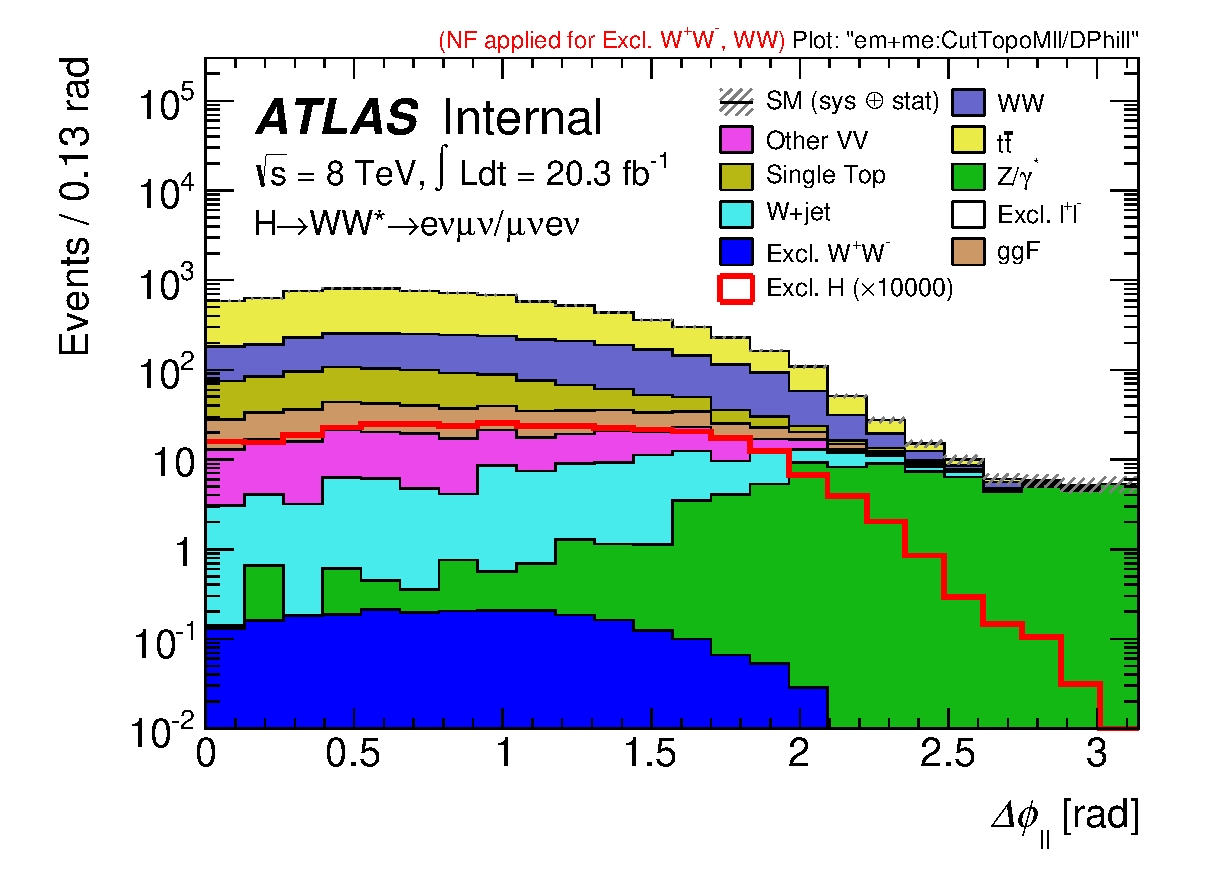
\includegraphics[width=0.5\linewidth]{emme_CutTopoMll_DPhill_mh125_log.eps}\\
\caption{\dfll distribution. The $\dfll<1.8$ cut reduces Drell Yan and WW backgrounds while 
keeping 90\% of signal.}
\label{fig:dphill}
\end{figure}

\par Table~\ref{table:sr} summarizes the selection criteria for signal events. Signal, ggF and WW yields 
are estimated at each cut level. {\it Blinding} refers to all the pre-selection cuts. The rest of the cuts
listed in the table are self-explanatory. Additional exclusivity cuts are imposed on Higgs-like events to 
select exclusive Higgs events. These will be discussed in Section~\ref{section:exclusivity}. Signal yields 
have been scaled by 100.

\begin{table}
\begin{center}
        \resizebox{0.9\textwidth}{!}{
\begin{tabular}{l||rrrr}
Cut & Excl. H & ggF H & $WW$ & Excl. $W^{+}W^{-}$ \\
\hline\hline
\textcolor{blue}{Scale factors} & \color{blue}NF = 100.00 &  &  &  \\
 blinding & 6.99 $\pm$ 0.05 & 585.63 $\pm$ 1.00 & 11641.95 $\pm$ 18.53 & 6.49 $\pm$ 0.03 \\
lepton $p_{\mathrm{T}}$ 25, 15 GeV & 4.59 $\pm$ 0.04 & 434.84 $\pm$ 0.86 & 10657.89 $\pm$ 17.79 & 5.84 $\pm$ 0.03 \\
OS leptons & 4.59 $\pm$ 0.04 & 434.23 $\pm$ 0.86 & 10618.52 $\pm$ 17.76 & 5.82 $\pm$ 0.03 \\
$m_{\ell\ell} > 10$ GeV & 4.52 $\pm$ 0.04 & 430.02 $\pm$ 0.86 & 10606.74 $\pm$ 17.75 & 5.82 $\pm$ 0.03 \\
$\met,\metRel > 20, 25$ GeV & 4.27 $\pm$ 0.04 & 358.80 $\pm$ 0.78 & 8494.57 $\pm$ 15.88 & 5.23 $\pm$ 0.03 \\
$\Delta\phi_{\ell\ell, MET} > 1.57$ & 4.27 $\pm$ 0.04 & 318.16 $\pm$ 0.74 & 7590.42 $\pm$ 15.01 & 5.22 $\pm$ 0.03 \\
$p_{\mathrm{T},\ell\ell}>$30 GeV & 3.83 $\pm$ 0.04 & 285.01 $\pm$ 0.70 & 6183.69 $\pm$ 13.54 & 4.63 $\pm$ 0.03 \\
$m_{\ell\ell}<55$ GeV & 3.28 $\pm$ 0.03 & 246.08 $\pm$ 0.65 & 1578.43 $\pm$ 6.80 & 0.81 $\pm$ 0.01 \\
$\Delta\phi_{\ell\ell}<1.8$ & 2.98 $\pm$ 0.03 & 231.26 $\pm$ 0.63 & 1462.57 $\pm$ 6.54 & 0.77 $\pm$ 0.01 \\
\hline
Exclusivity Cuts & & & &
\end{tabular}
}
\caption{Signal selection criteria. {\it Blinding} refers to all the pre-selection cuts. Yields are normalized to 20.3\ifb and 
signal is scaled by a normalization/scale factor (NF) of 100.}
\label{table:sr}
\end{center}
\end{table}

%%%%%%%%%%%%%%%%%%%%

%%%%%%%%%%%%%%%%%%%%
\clearpage
\section{Exclusivity }
\label{sec:exclusivity}

\par With the high pileup environment in 8 TeV data it is crucial to improve
on what has been done with 7 TeV data~\cite{CMSmumu}~\cite{CMSee}~\cite{MonteNote}.
With 8 TeV data, the strategy adopted at 7 TeV of requiring a 2-track vertex
and not having another track within 3 mm is only 30\% efficient. This strategy 
 is unreliable because the vertexing algorithms can be overly enthusiastic about 
associating tracks to a vertex. As a result, originally 2-track
vertices are assigned 3 or more tracks.   

\subsection{Strategy}
\par The strategy used at 8 TeV is to demand that the lepton pair not have any tracks
other than those from the two leptons within a window in~\z0\ along 
the beamline. Tracks are taken from the trk container and required to have 
at least 1 pixel hit and at least 4 sct hits. In contrast, lepton tracks are taken 
from the lepton containers. It is therefore necessary to match the lepton tracks to two tracks from the trk container.
For a track in the trk container to be considered a match to a lepton track it is required to
be within 0.01 in $\Delta R$ and within 1 mm  in \z0, with respect to 
the beamline. The tracks in the electron or muon
containers are obtained using algorithms (GSM) different from the algorithms
used in the trk container. For this reason, a lepton track may not be matched to a track in the trk container
or may be matched to multiple tracks in the trk container. Figure~\ref{fig:trackMatching} 
shows the number of tracks from the trk container that match the leading lepton 
in the event. The distribution on the left is for matching tracks to an electron and 
that on the right is for matching tracks to muons. 
 
\begin{figure}[!h]
\centering
\begin{tabular}{c}
	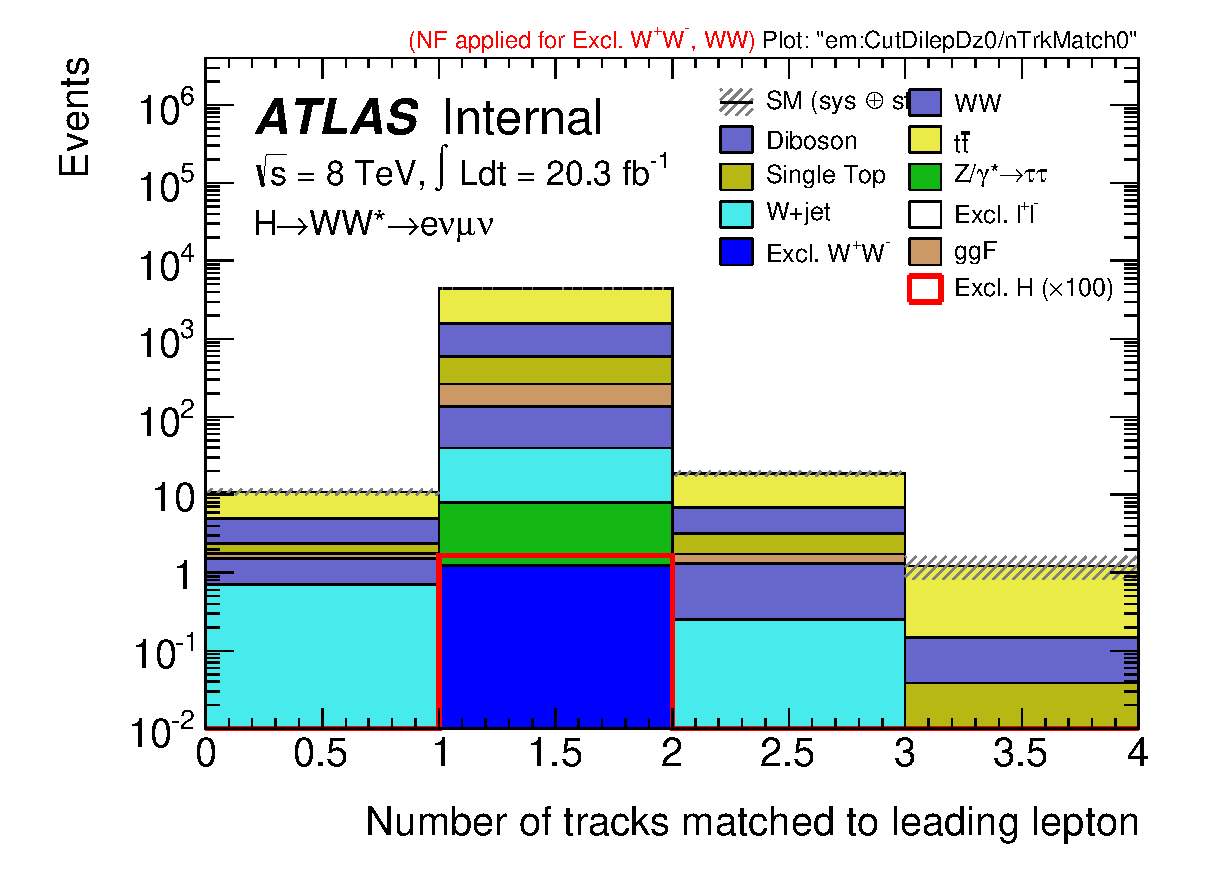
\includegraphics[width=0.5\linewidth]{em_CutDilepDz0_nTrkMatch0_mh125_log.eps}
	\includegraphics[width=0.5\linewidth]{me_CutDilepDz0_nTrkMatch0_mh125_log.eps}\\
\end{tabular}
\caption{Number of tracks from the trk container that are matched to the leading 
lepton tracks. [Left] The leading lepton is an electron. [Right] The leading lepton 
is a muon.}
\label{fig:trackMatching}
\end{figure}

\par Because electrons undergo bremsstrahlung more frequently than muons, there are more tracks 
matched to electrons than to muons. All the tracks matched to a lepton are therefore 
considered to be brehming from that lepton.

\par The exclusivity cut depends on how far in \z0\ the closest unmatched track 
is from the lepton track pair. Figure~\ref{fig:cartoon} illustrates how this is quantified. 
The two lepton tracks are first required to be within 1 mm in \z0\ to ensure that they indeed 
are from the lepton pair. The average \z0\ position computed from the individual lepton track \z0's is 
considered the dilepton vertex. The distance of the closest unmatched track $\Delta z_1$ is the 
exclusivity variable that is cut on. Figure~\ref{fig:deltaZ1} shows $\Delta z_1$  for signal and several backgrounds.
The signal is scaled by a factor of 100 to make it visible because it is heavily dominated by the backgrounds.
The $\Delta z_1$ distribution in signal and other exclusive processes 
is characterized by a tail more spread out than in inclusive processes. Several values of $\Delta z_1$ 
were tried to maximize $signal/\sqrt{background}$. Figure~\ref{fig:sOverB} shows $signal/\sqrt{background}$
for four values of $\Delta z_1$. This analysis settles on $\Delta z_1 > 1 mm$ as the optimal 
exclusivity cut.    

\begin{figure}[t]
\centering
\includegraphics[width=0.4\linewidth]{cartoon.eps}
\caption{Illustration of the exclusivity variables.}
\label{fig:cartoon}
\end{figure}

\begin{figure}[!h]
\centering
\begin{tabular}{c}
	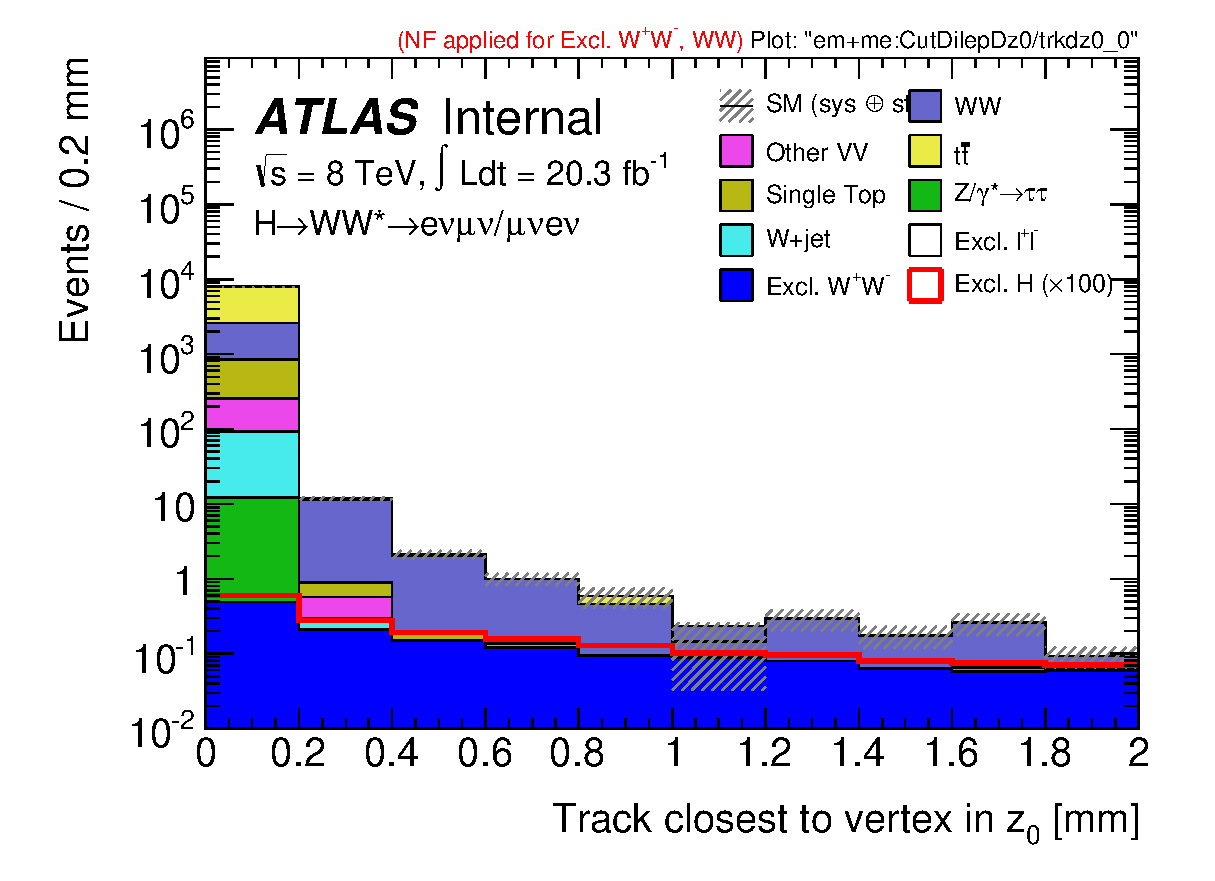
\includegraphics[width=0.5\linewidth]{trkdz0_deltaZ1.eps}
\end{tabular}
\caption{The main exclusivity variable $\Delta z_1$, which is the distance of 
the closest unmatched track to the dilepton vertex in \z0. Signal is scaled by 100. 
$\Delta z_1$ has a longer tail in exclusive processes compared to inclusive processes. 
This distrinction is exploited in this study.}
\label{fig:deltaZ1}
\end{figure}

\begin{figure}[!h]
\centering
\begin{tabular}{c}
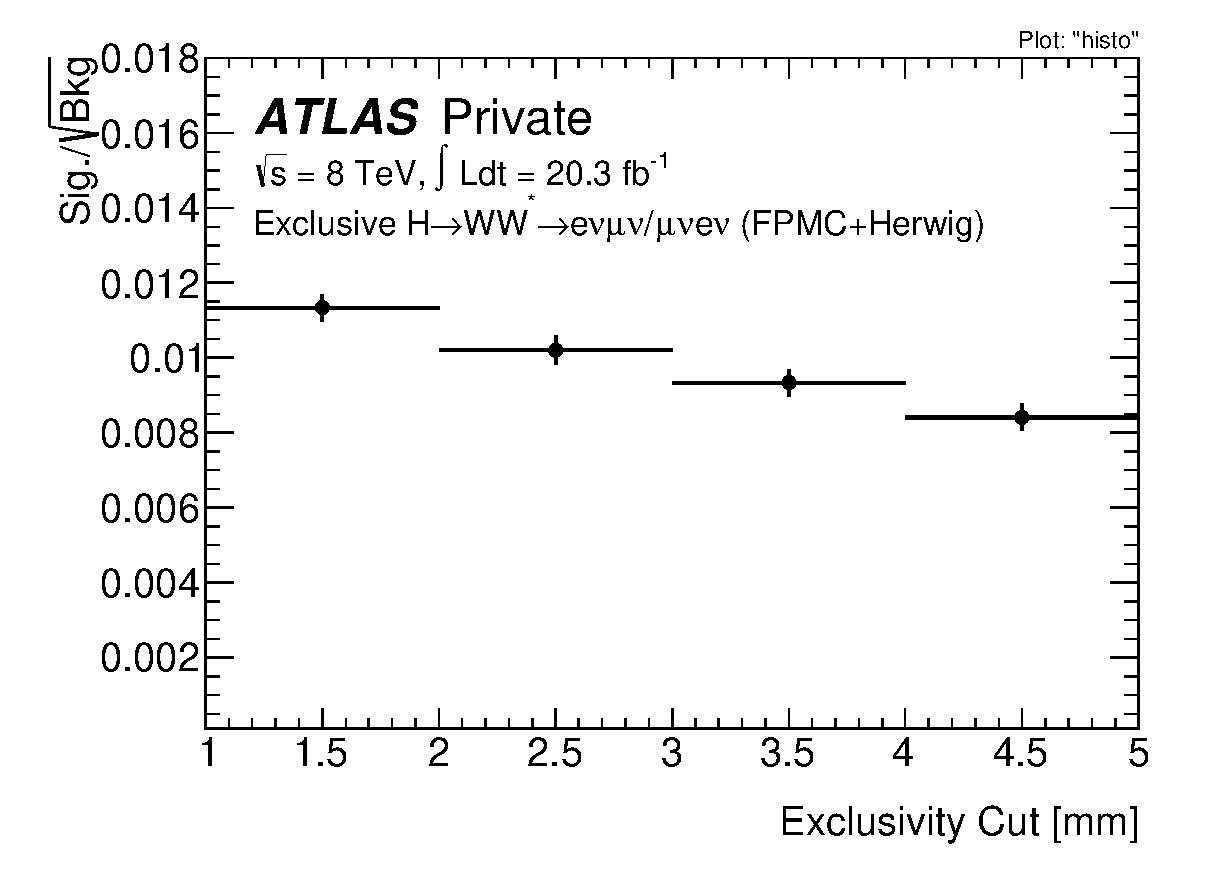
\includegraphics[width=0.7\linewidth]{emme_sOverB.eps}
\end{tabular}
\caption{$signal/\sqrt{background}$ for 4 values of $\Delta z_1$. This analysis settles 
on $\Delta z_1 > 1 mm$ as the optimal exclusivity cut.}
\label{fig:sOverB}
\end{figure}

\subsection{Performance in data}
\par A region in data that is rich in \Ztau\ events is used to validate the exclusivity selection 
criteria. This region follows the control region used in Ref.~\cite{ATLASCONF2014060} to constrain 
 \Ztau+0-jets events in the \HWW\ study. In this study we apply it to any jet multiplicity.
The selection is similar to the signal selection criteria except the following: \mll\ region is expanded to 
cover $10<\mll<80 $GeV, \ptll\ is changed to $\ptll<30 $GeV. There is no \dfll\ cut. Figure~\ref{fig:ztauCR}
shows some kinematic distributions of events in this \Ztau\ region. Before exclusivity, MC over-estimate 
\Ztau\ yields by 0.3\% in this region. After exclusivity MC over-estimate the yield by 387\%.
This is because MC mismodeles the underlying event. Table~\ref{table:ztauCR} shows the event yields in both
data and MC. Figure~\ref{fig:ztauCR} shows key kinematic distributions before exclusivity is imposed 
in this control region. The good agreement between data and MC testify to the purity of the \Ztau\ events
in data.  

\begin{table}
\centering
        \resizebox{.6\textwidth}{!}{
\begin{tabular}{l||r|rr}
 & $Z+\gamma/$jets & Observed & Data/MC \\
\hline\hline
blinding & 34360.39 $\pm$ 473.93 & 92352 & 1.19 $\pm$ 0.01 \\
lepton $p_{\mathrm{T}}$ & 17990.93 $\pm$ 346.30 & 62517 & 1.12 $\pm$ 0.01 \\
OS leptons & 17821.85 $\pm$ 344.56 & 60072 & 1.10 $\pm$ 0.01 \\
$m_{\ell\ell} > 10$ GeV & 17803.29 $\pm$ 344.32 & 60002 & 1.10 $\pm$ 0.01 \\
$E^{\mathrm{miss}}_{\mathrm{T,rel}} < 25$ GeV & 13722.36 $\pm$ 300.23 & 28896 & 1.08 $\pm$ 0.01 \\
$\Delta\phi_{\ell\ell, MET} > 1.57$ & 11127.20 $\pm$ 270.22 & 19390 & 1.04 $\pm$ 0.02 \\
$p_{\mathrm{T},\ell\ell}<$30 GeV & 10908.72 $\pm$ 267.29 & 12060 & 0.98 $\pm$ 0.02 \\
$m_{\ell\ell}<80$ GeV & 10651.88 $\pm$ 264.46 & 10600 & 0.95 $\pm$ 0.02 \\
$\Delta z^{0}_{ll}<1.0$ mm & 10576.86 $\pm$ 263.56 & 10538 & 0.95 $\pm$ 0.02 \\
\hline
1 mm Exclusive & 58.38 $\pm$ 19.86 & 12 & 0.21 $\pm$ 0.09 \\
\end{tabular}
}
\label{table:ztauCR}
\caption{\Ztau\ yields in the \Ztau\ control region. Right before exclusivity is imposed, MC over-estimate 
\Ztau\ yields by 0.3\%. After exclusivity, the over-estimation rises to 387\%.}
\end{table}


\begin{figure}[!h]
\centering
\begin{tabular}{c}
	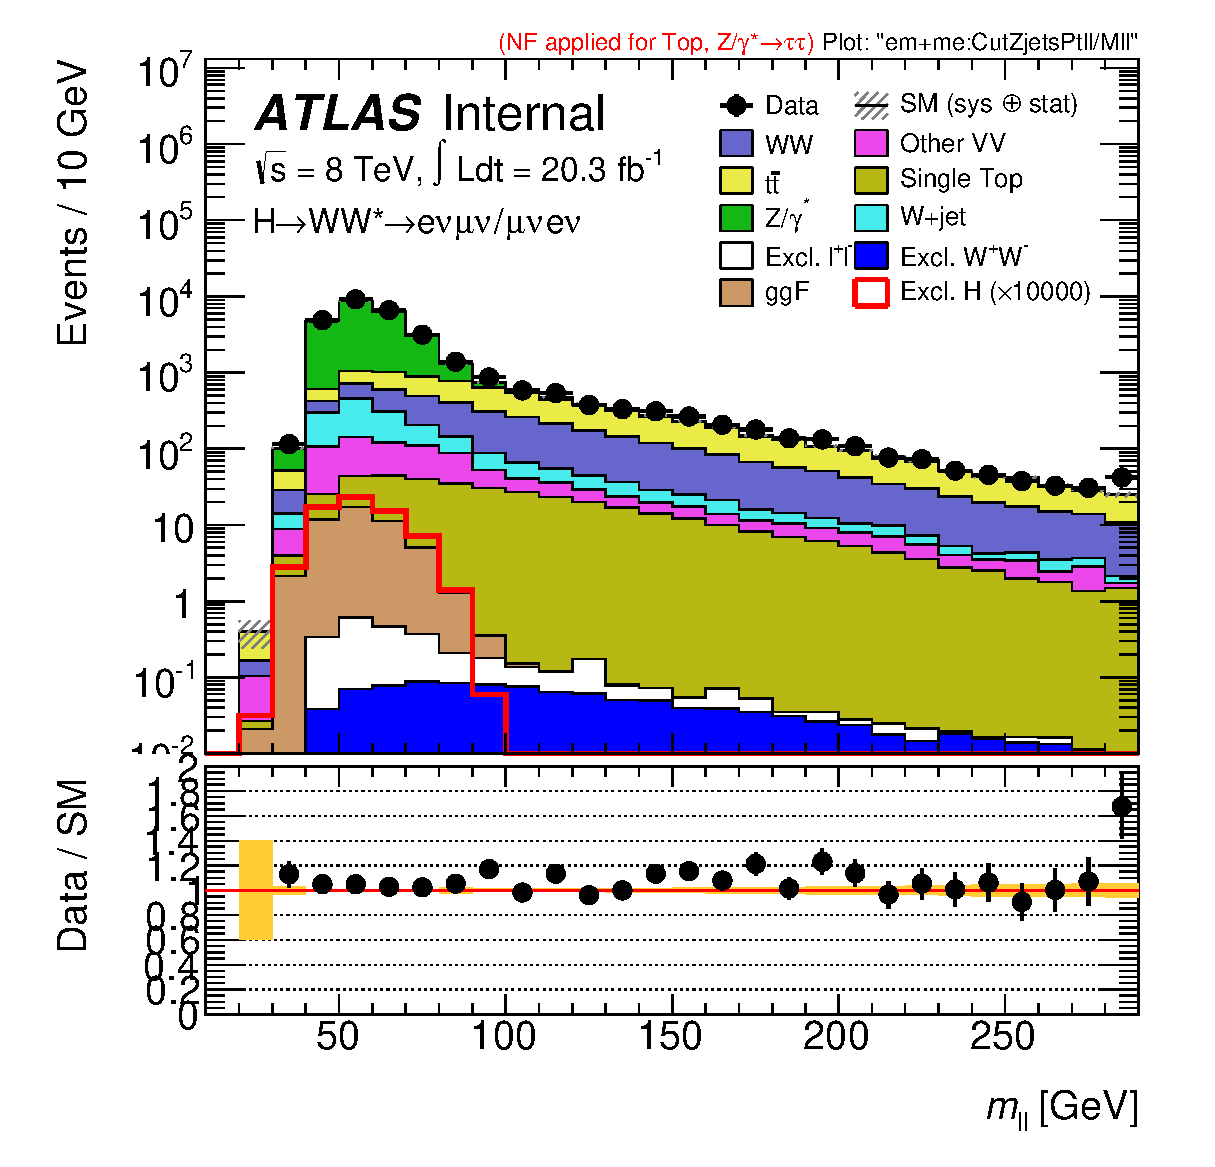
\includegraphics[width=0.5\linewidth]{emme_CutZjetsPtll_Mll_mh125_log.eps}
	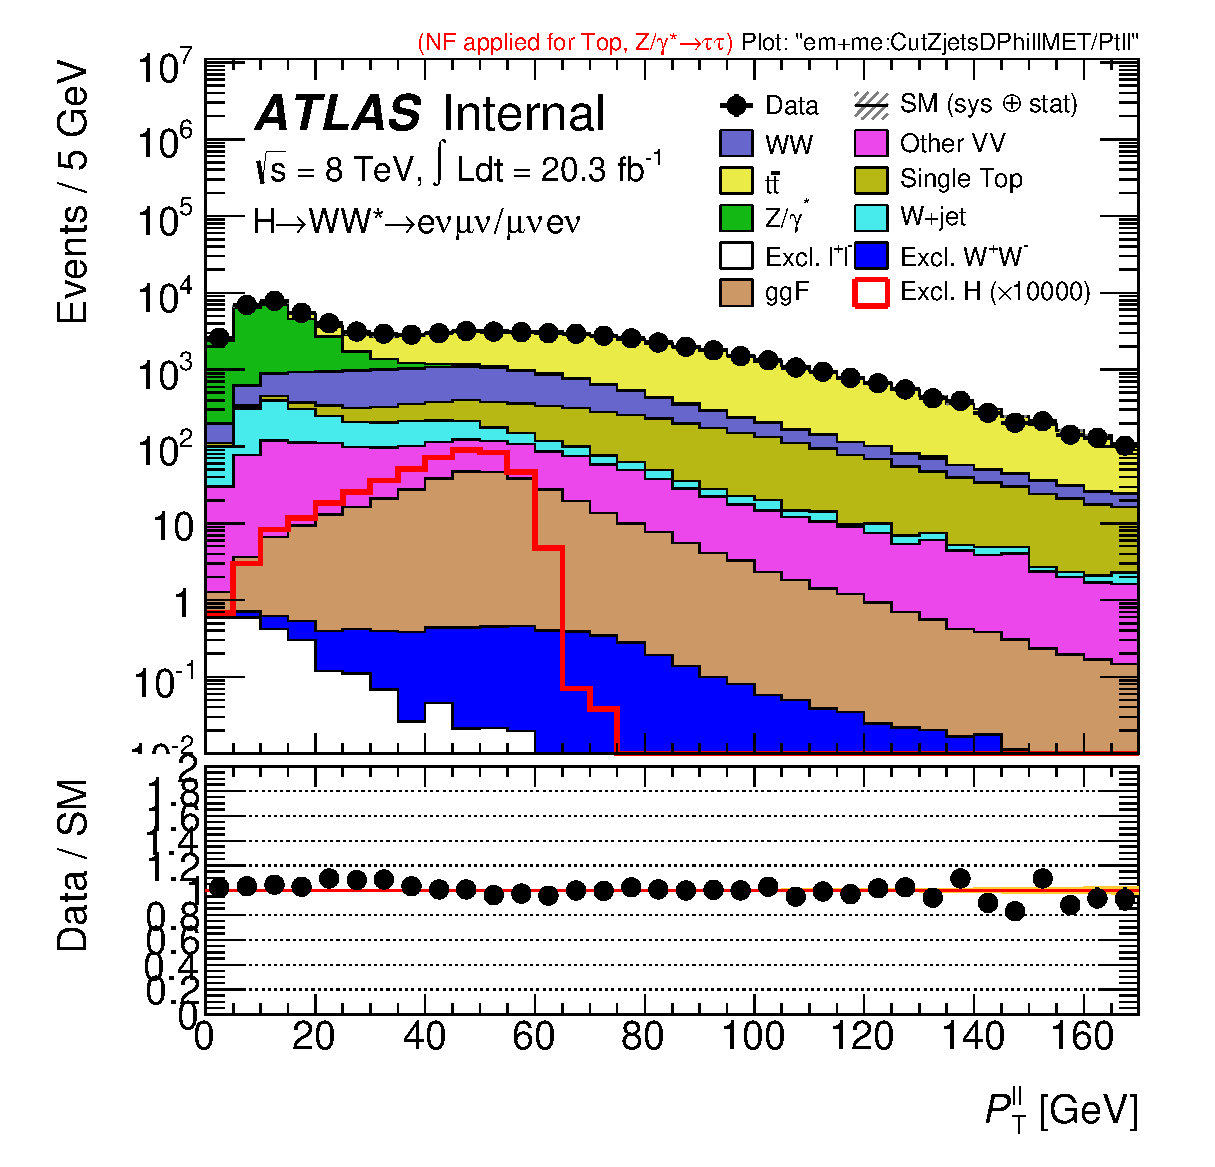
\includegraphics[width=0.5\linewidth]{emme_CutZjetsDPhillMET_Ptll_mh125_log.eps}\\
	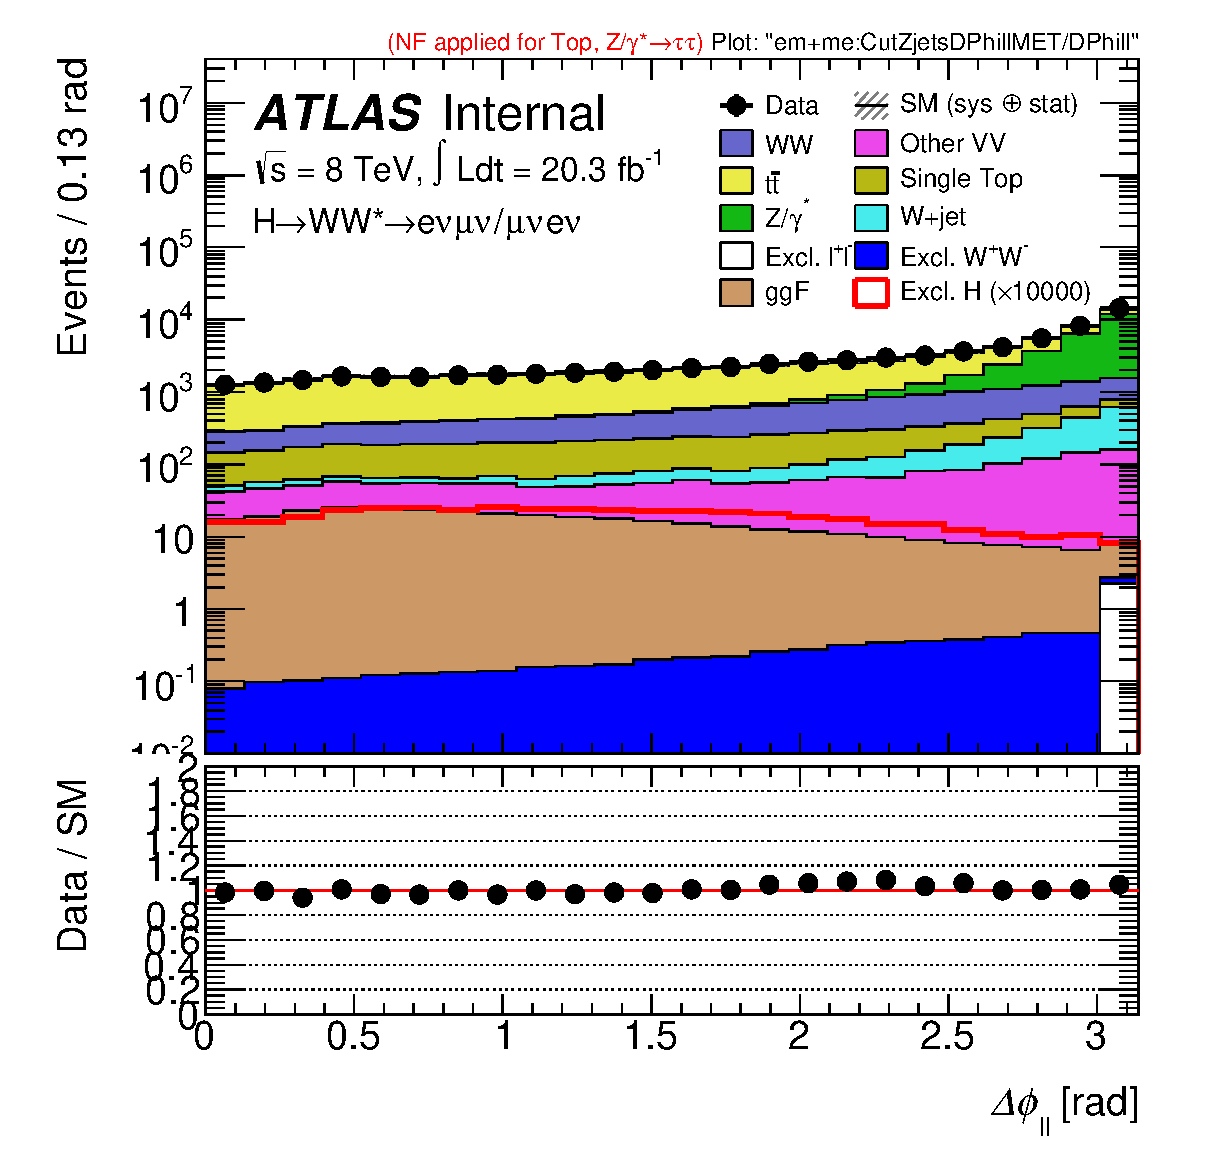
\includegraphics[width=0.5\linewidth]{emme_CutZjetsDPhillMET_DPhill_mh125_log.eps}
	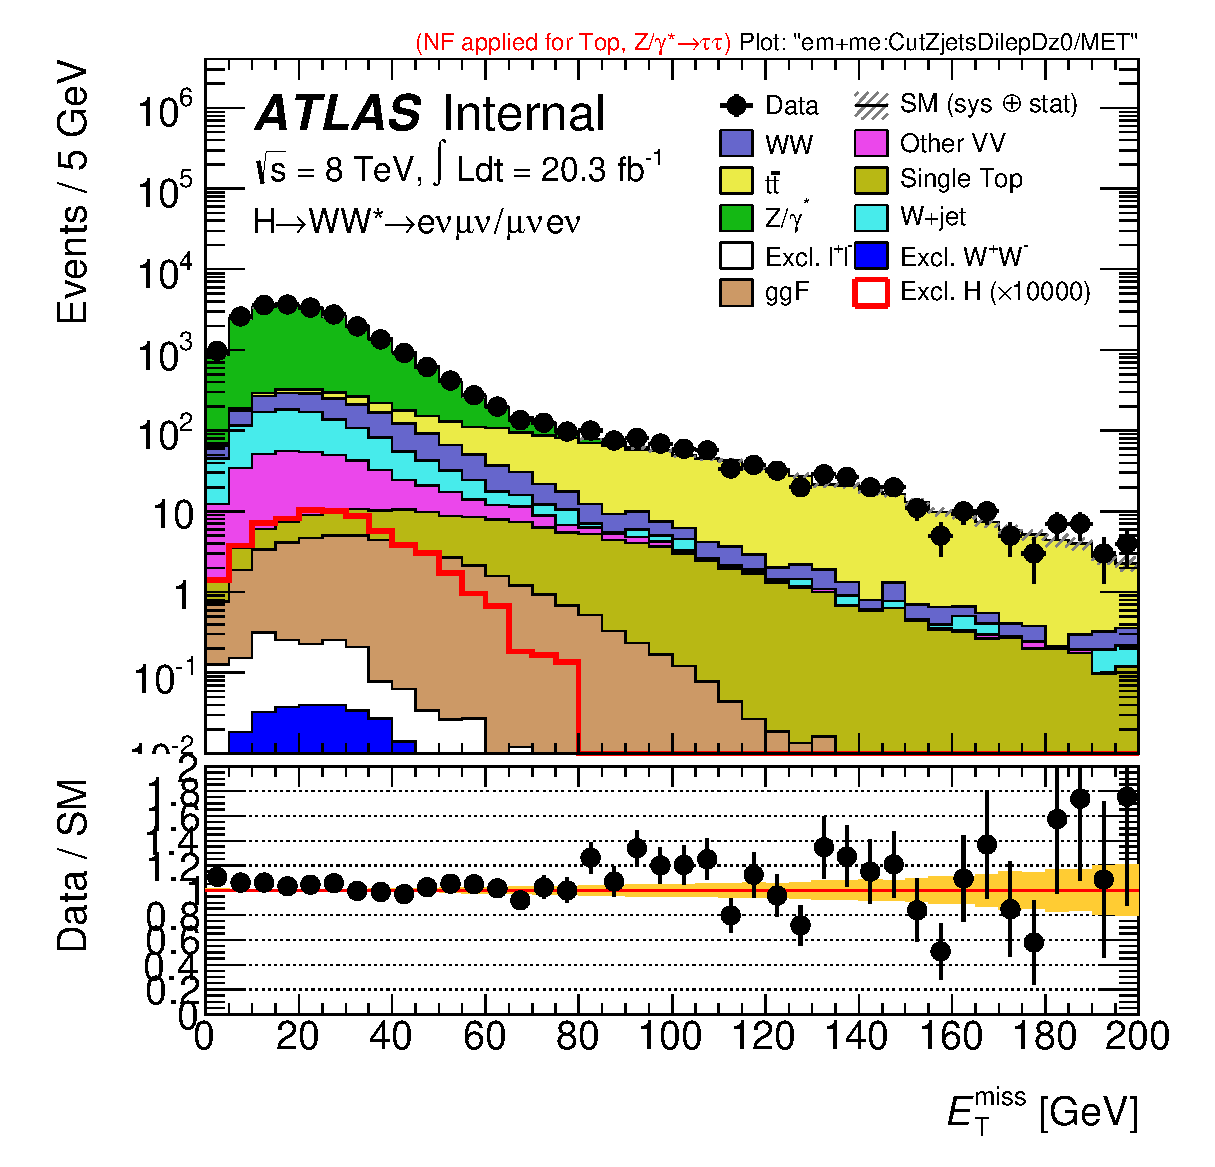
\includegraphics[width=0.5\linewidth]{emme_CutZjetsDilepDz0_MET_mh125_log.eps}\\
	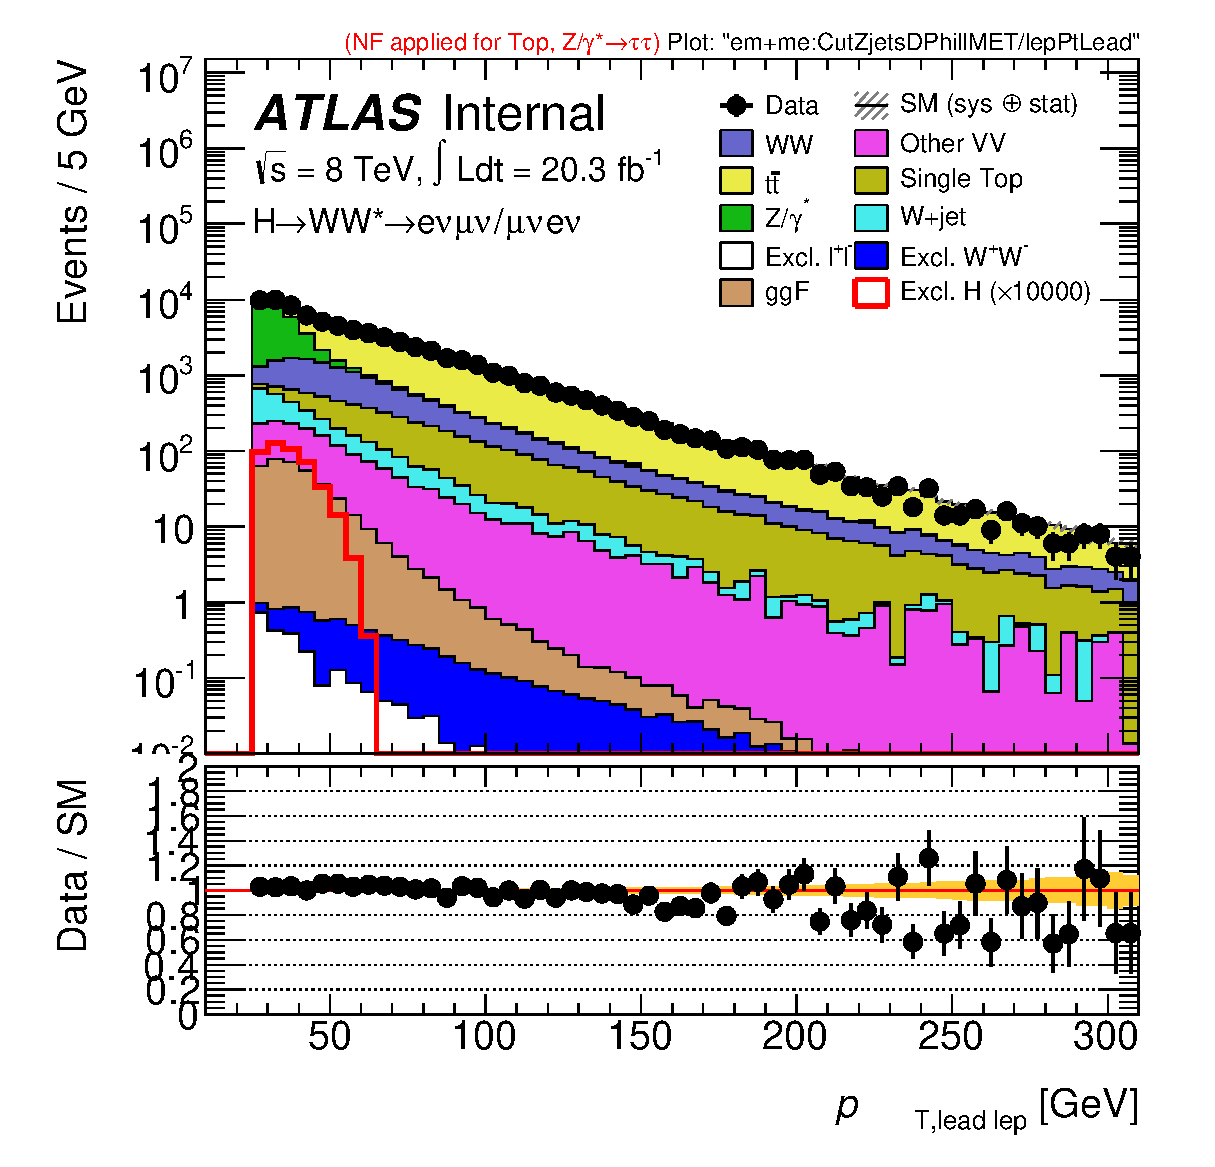
\includegraphics[width=0.5\linewidth]{emme_CutZjetsDPhillMET_lepPtLead_mh125_log.eps}
	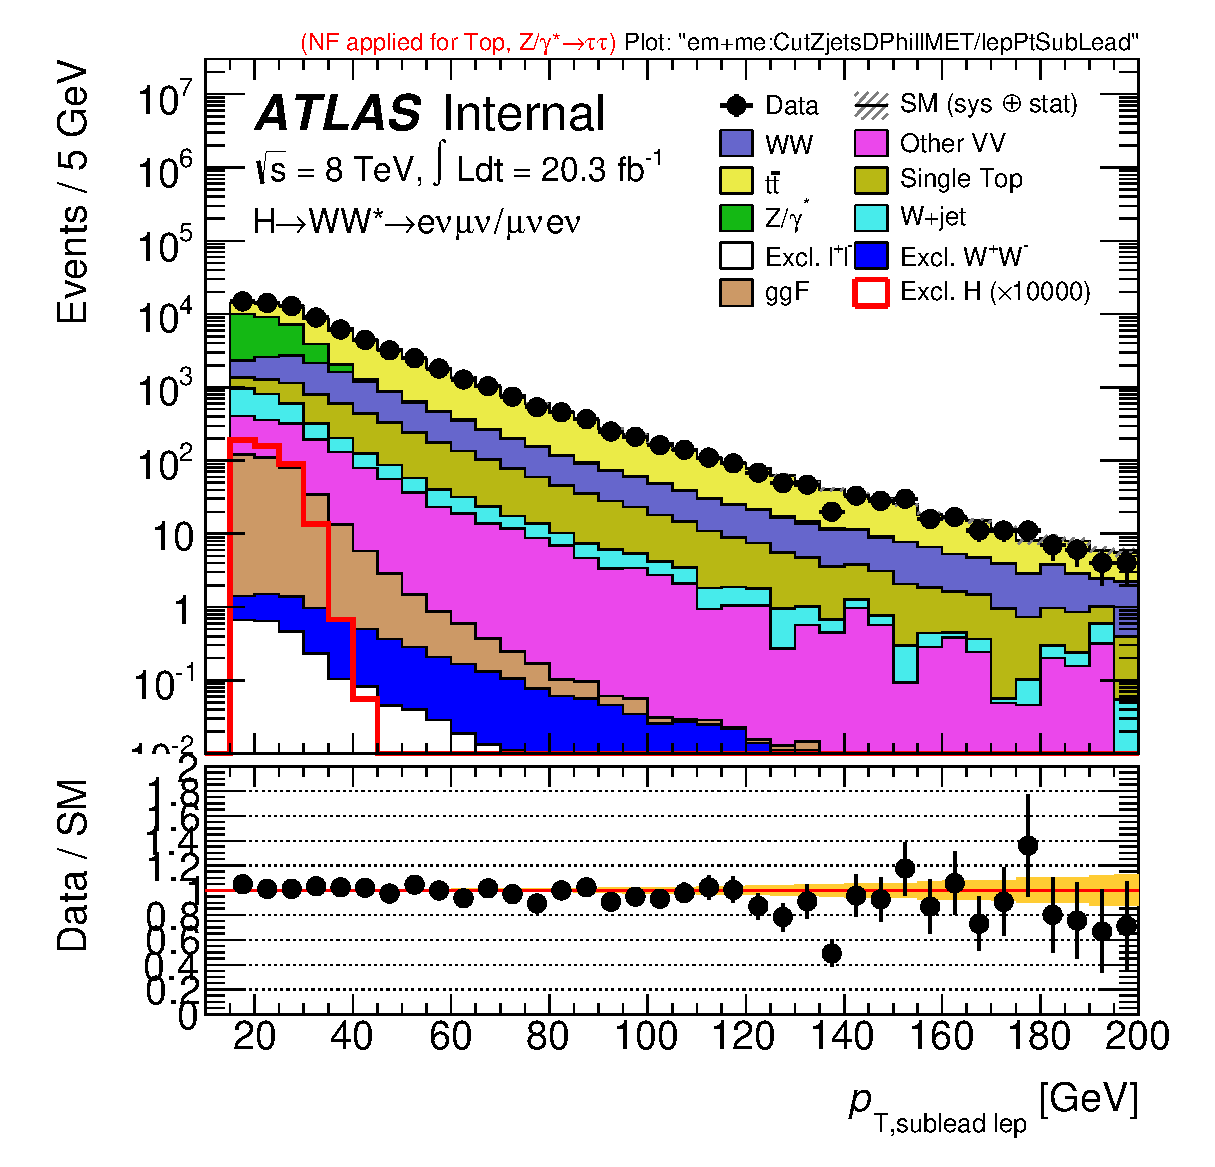
\includegraphics[width=0.5\linewidth]{emme_CutZjetsDPhillMET_lepPtSubLead_mh125_log.eps}\\
\end{tabular}
\caption{Key kinematic distributions in the \Ztau\ control region before the exclusivity cut is imposed.}
\label{fig:ztauCR}
\end{figure}

\par Figure~\ref{figztauExclCR} shows distributions for exclusivity variables before the exclusivity cut is imposed.
The difference in $z_0$ between the two lepton tracks is also affected by the underlying event. The $\Delta z_1$
distribution shows a uniform disagreement between data and MC for $\Delta z_1>1$ mm. This disagreement results in the 
387\% data/MC disagreement alluded to in the preceding paragraph. To correct for this we introduce  a correction factor, 

\begin{equation}
\mbox{MC Exclusivity Correction Factor, MF} = \frac{N^{mc}_{after\ excl.}/N^{mc}_{before\ excl.}}{N^{data}_{after\ excl.}/N^{data}_{before\ excl.}}
\end{equation}

which is the ratio of the exclusivity cut efficiency in MC to its efficiency in data.
Ideally it is 1.0 if MC models the underlying event correctly. An MF larger than 1.0 implies that MC over-estimate
events that pass the exclusivity cut. The Alpgen+Jimmy MC that we use for this region give $MF=4.72$. 
 
\begin{figure}[!h]
\centering
\begin{tabular}{c}
	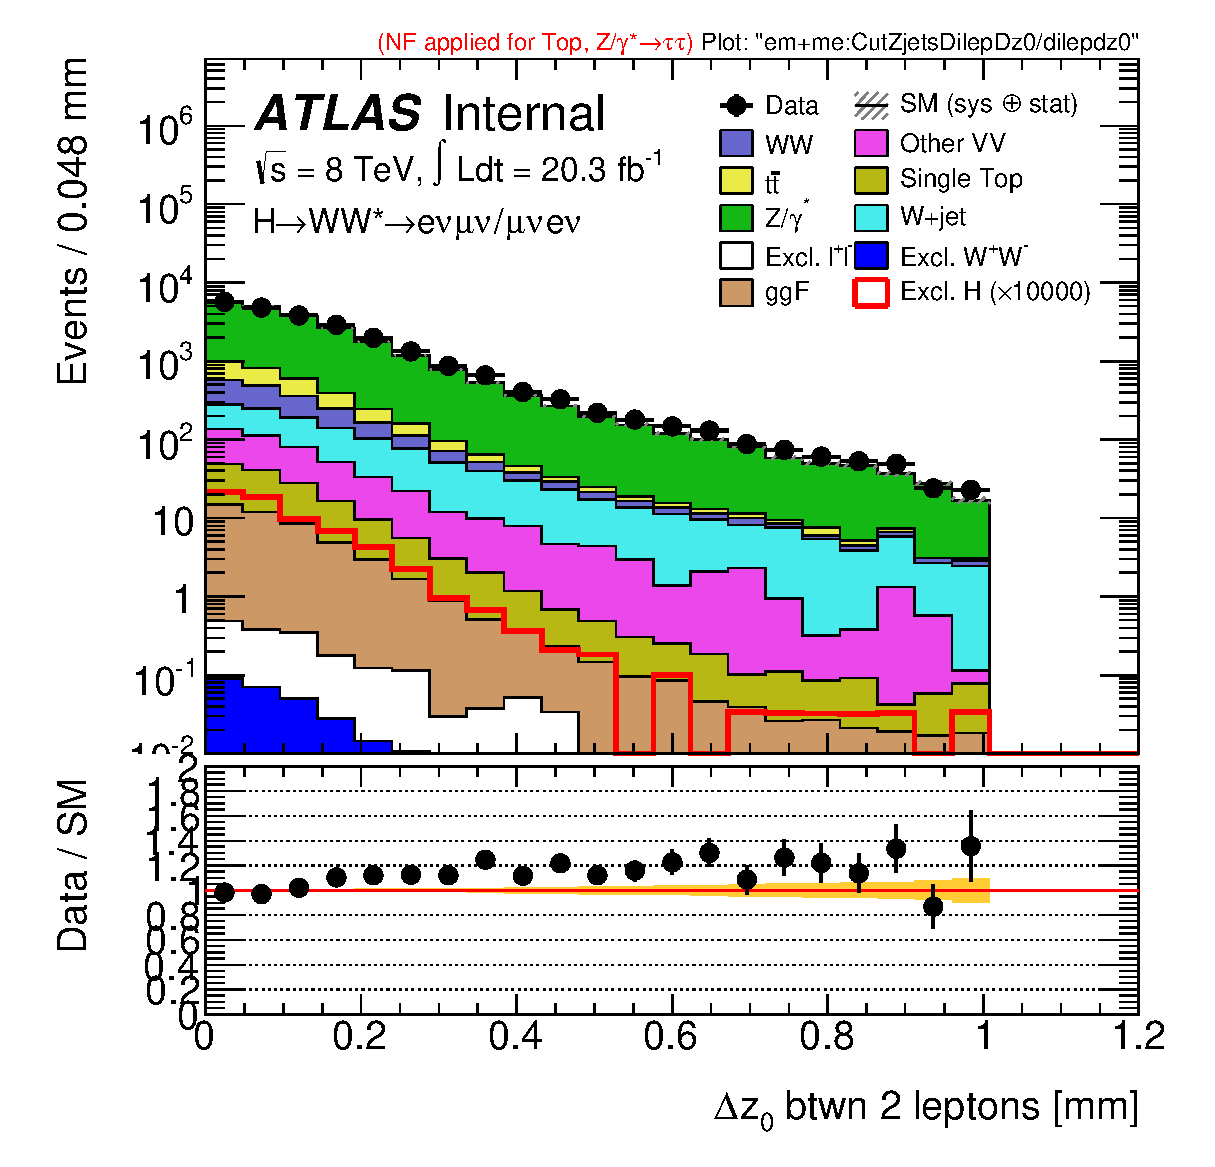
\includegraphics[width=0.5\linewidth]{emme_CutZjetsDilepDz0_dilepdz0_mh125_log.eps}
	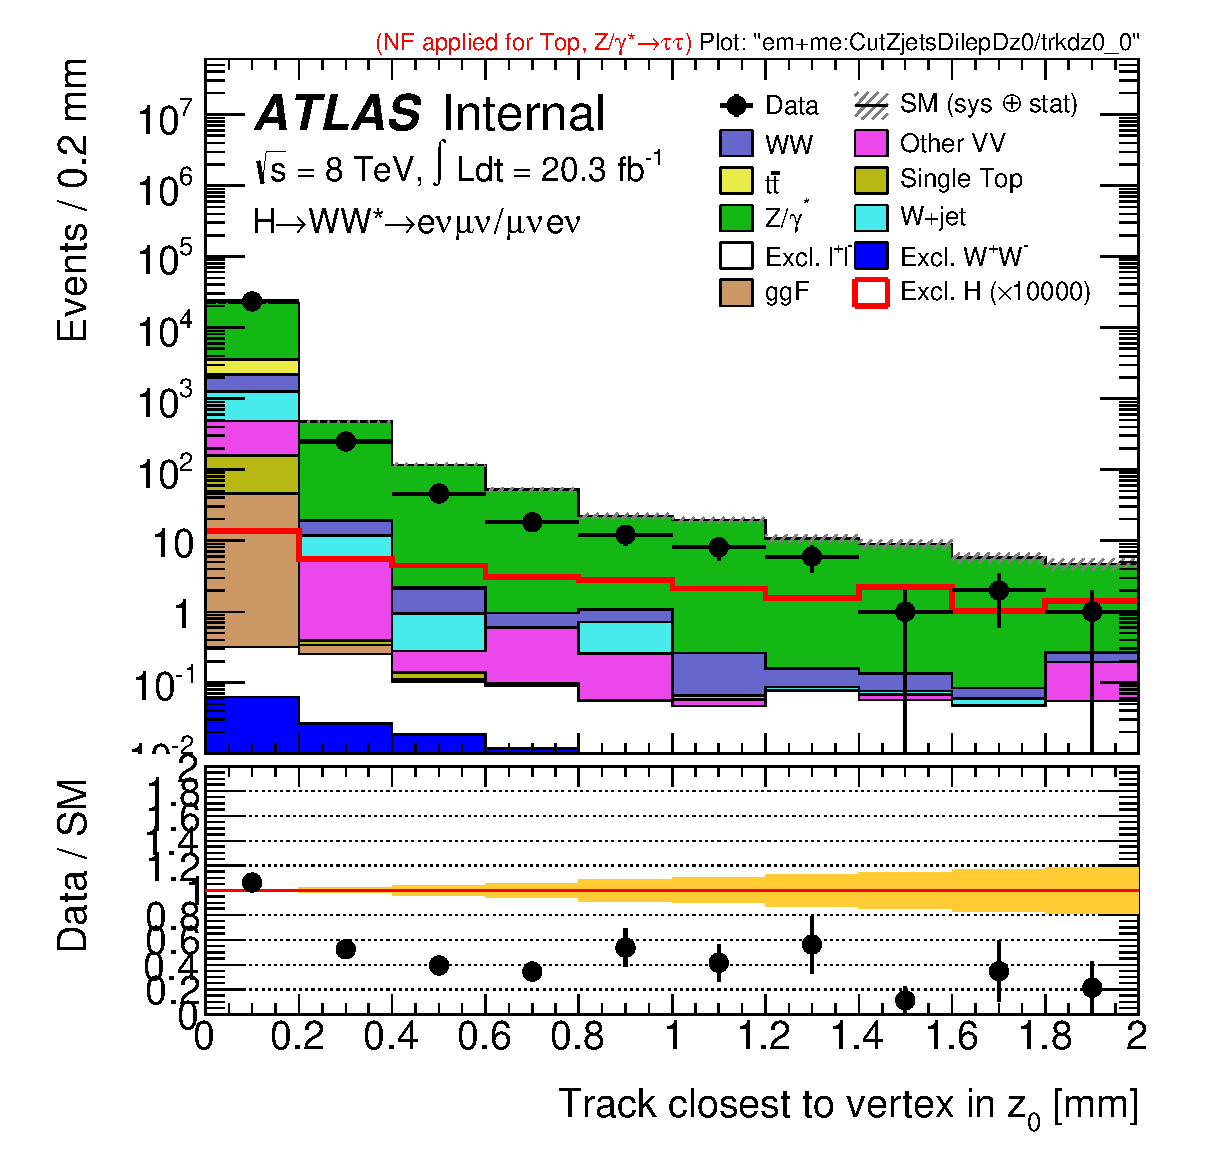
\includegraphics[width=0.5\linewidth]{emme_CutZjetsDilepDz0_trkdz0_0_mh125_log.eps}\\
\end{tabular}
\caption{Exclusivity variables in the \Ztau\ control region show a disagreement between data and MC. This
motivates the use of a correction factor on the MC.}
\label{fig:ztauExclCR}
\end{figure}

\par Studies similar to the \Ztau\ study were done using \Zmm\ events, estimating them 
with several MC listed in Table~\ref{table:mf}. The resulting MFs are listed in the same table.
All MC studied tend to over-estimate events that pass the exclusivity cut. Of all these MC,
Sherpa over-estimates the most. Figure~\ref{fig:mf} shows the number of tracks within a 1.0 mm
around the di-muon vertex, computed as shown in Figure~\ref{fig:cartoon}. The exclusivity cut select 
only the events that are in the first bin of these plots. Clearly Sherpa over-estimates these 
events by a factor close to 10 (9.23 to be precise). Because this analysis relies heavily on 
MC to estimate major backgrounds, it is necessary to correct the MC using MFs. By comparing the 
Alpgen+Jimmy MF obtained using \Zmm\ events to the one obtained using \Ztau\ events we notice 
that they agree within 8\%. Clearly the MF is a major source of systematic uncertainties. We will 
discuss these in Section~\ref{sec:syst}.  

\begin{table}
\begin{center}
        \resizebox{0.4\textwidth}{!}{
\providecommand{\cutflowTitle}{hsg3}
\begin{tabular}{l|rr}
 & \Zmm & \Ztau   \\
\hline\hline
Sherpa &       9.23 &  \\
AlpgenPythia & 1.65 & \\
AlpgenJimmy & 4.36  & 4.72\\
PowhegPythia & 2.35 & 
\end{tabular}
}
\caption{MFs obtained from studying \Zmm\ and \Ztau\ events and estimating them using several MC. Sherpa 
mismodels the underlying event the worst. We use Alpgen+Jimmy MC in this analysis.}
\label{table:mf}
\end{center}
\end{table}

\begin{figure}[!h]
\begin{tabular}{c}
	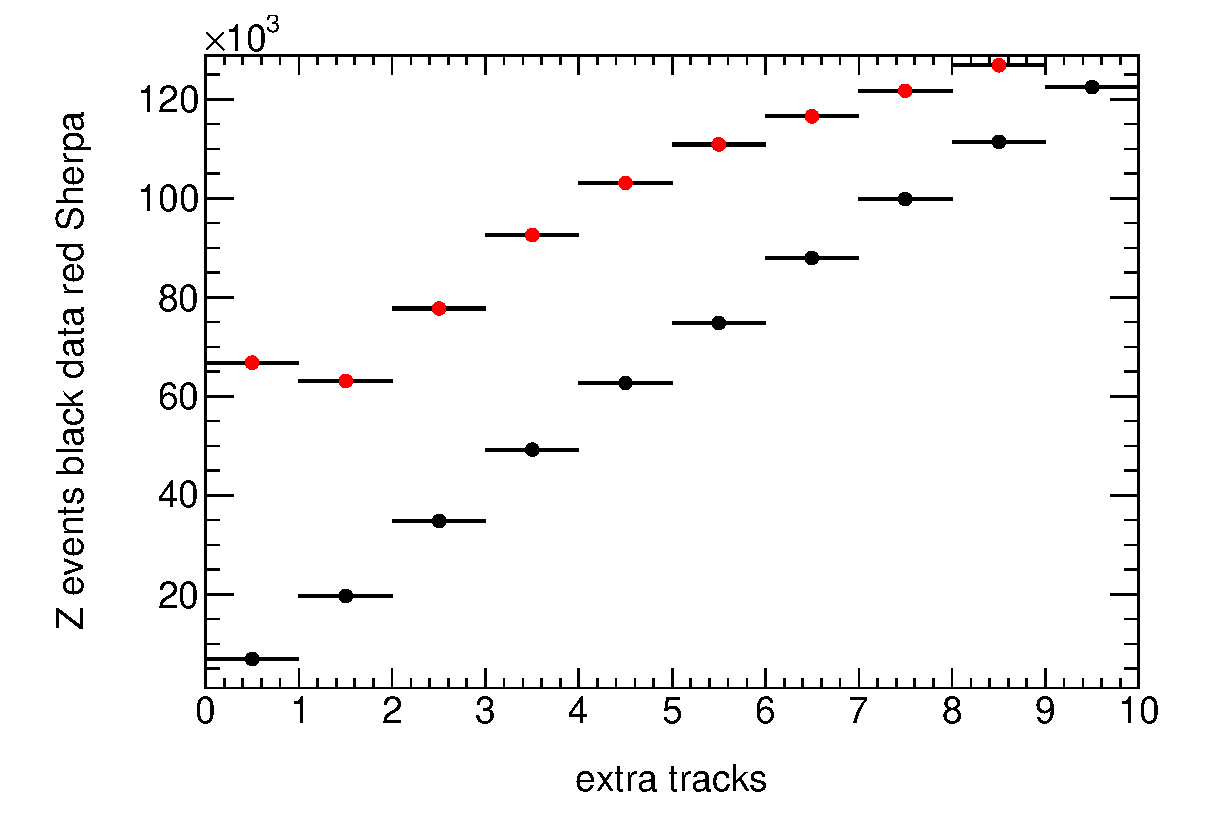
\includegraphics[width=0.5\linewidth]{extraZsherpa.eps}
	\includegraphics[width=0.5\linewidth]{extraZpowheg.eps}
\end{tabular}
\caption{Number of extra tracks within a 1.0 mm window around the di-muon vertex calculated as 
shown in Figure~\ref{fig:cartoon}. Events that pass exclusivity cut are in the first bin of these plots.
Sherpa clearly is the worst at modelling the underlying event. }
\label{fig:mf}
\end{figure}

%%%%%%%%%%%%%%%%%%%%
%
%%%%%%%%%%%%%%%%%%%%
\clearpage
\section{Background Estimation}
\label{sec:bkgEst}

\subsection{Exclusive WW}
\par As shown at the end of Section~\ref{sec:theory} there are three diagrams that contribute 
to the exclusive WW process. Although Herwig++ models the purely elactic events well, there are 
no MC that model SD and DD processes. To estimate the SD and DD contributions we study di-muon
events in data that pass the exclusivity cut and that have $\mll>160$ GeV to reduce di-muons 
from WW decays and Drell-Yan. The remaining Drell-Yan contribution in this region is estimated 
with MC and subtracted. All other backgrounds are considered as well but the major contributions are observed 
to be from inclusive WW, exclusive WW and Drell-Yan. Inclusive WW and Drell-Yan estimations 
are scaled with appropriate MFs to account for the MC mismodelling of the underlying event.
There is no need to apply MF to exclusive WW and exclusive di-muon estimates because there 
is no underlying event in these processes. 

\par After all the backgrounds are subtracted the remaining events are a good estimation of 
the sum of purely elastic, single dissociative and double dissociative di-muons. We introduce 
the

\begin{equation}
\mbox{Flux Factor} = \frac{N_{data} - N_{DY,etc}}{N_{elastic}}
\end{equation}

which quantifies the SD and DD contributions. Detailed studies concerning this factor can 
be found in Ref~\cite{CMSmumu}. A flux factor of 1.0 indicates that there is negligible SD 
and DD contributions to the exclusive di-muons. Table~\ref{table:flux} shows the results 
of studying di-muon events in data. A flux factor of $2.99\pm0.21$ is obtained, in which the 
uncertainty is only statistical. This shows that the SD and DD contributions are non-negligible.  

\begin{table}
\centering
        \resizebox{.4\textwidth}{!}{
\providecommand{\cutflowTitle}{hsg3}
\begin{tabular}{l|r}
\hline
 & Count \\
\hline\hline
Observed & 234 \\
Predicted Elastic $ll$ & 72.0 \\
MF-Scaled Drell-Yan & 16.2 \\
MF-Scaled Inclusive WW & 0.4 \\
MF-Scaled Exclusive WW & 0.82 \\
\hline
Flux Factor & $2.99\pm0.21$ \\
\end{tabular}
}
\caption{Results for the flux factor study on exclusive di-muons. A large flux factor 
implies that the contribution of SD and DD processes is non-negligible.}
\label{table:flux}
\end{table}

The diagrams that contribute to exclusive di-leptons are identical to the diagrams that contribute to 
exclusive WW. Thus, we can use the flux factor obtained from the di-muon study to estimate the 
SD and DD contributions in exclusive WW. We scale the Herwig++ estimation with 2.99 
to get the expected final exclusive WW yield, which turns out to be $1.25\pm0.02$. 

\subsection{Inclusive WW}
\par Inclusive WW are estimated using MC listed in Table~\ref{table:background}. A control region is 
used to assess the performance of these MC. The control region is defined as follows: Events that pass all 
the signal region cuts up to the $\ptll>30$ GeV cut are required to have $55<\mll<110$ GeV and 
$\dfll<2.6$ and have no jets. The 0-jet requirement suppresses \ttbar\ contribution. These selection criteria 
for this region are similar to the 0-jet WW control region detailed in Ref.~\cite{ATLASCONF2014060}. 
We notice that it is necessary to scale WW MC estimate by a factor of 1.22 to achieve data/MC agreement. 
This factor was also introduced in the \hwwll\ studies in Ref.~\cite{ATLASCONF2014060}. 
The exclusivity cut is then imposed after all these requirements are fulfilled and the scale 
factor has been applied.
Figure~\ref{fig:wwCR} shows key kinematic distributions in this control region after scaling MC with 1.22.
Table~\ref{table:wwCR} shows the corresponding MC estimated yields and observed event yields.
Figure~\ref{fig:exclwwCR} shows the $\Delta z_1$ distribution after applying the 1.22 scale factor on 
the inclusive WW, an MF on the inclusive WW and a flux factor on the exclusive WW processes.

\begin{figure}[!h]
\centering
\begin{tabular}{c}
	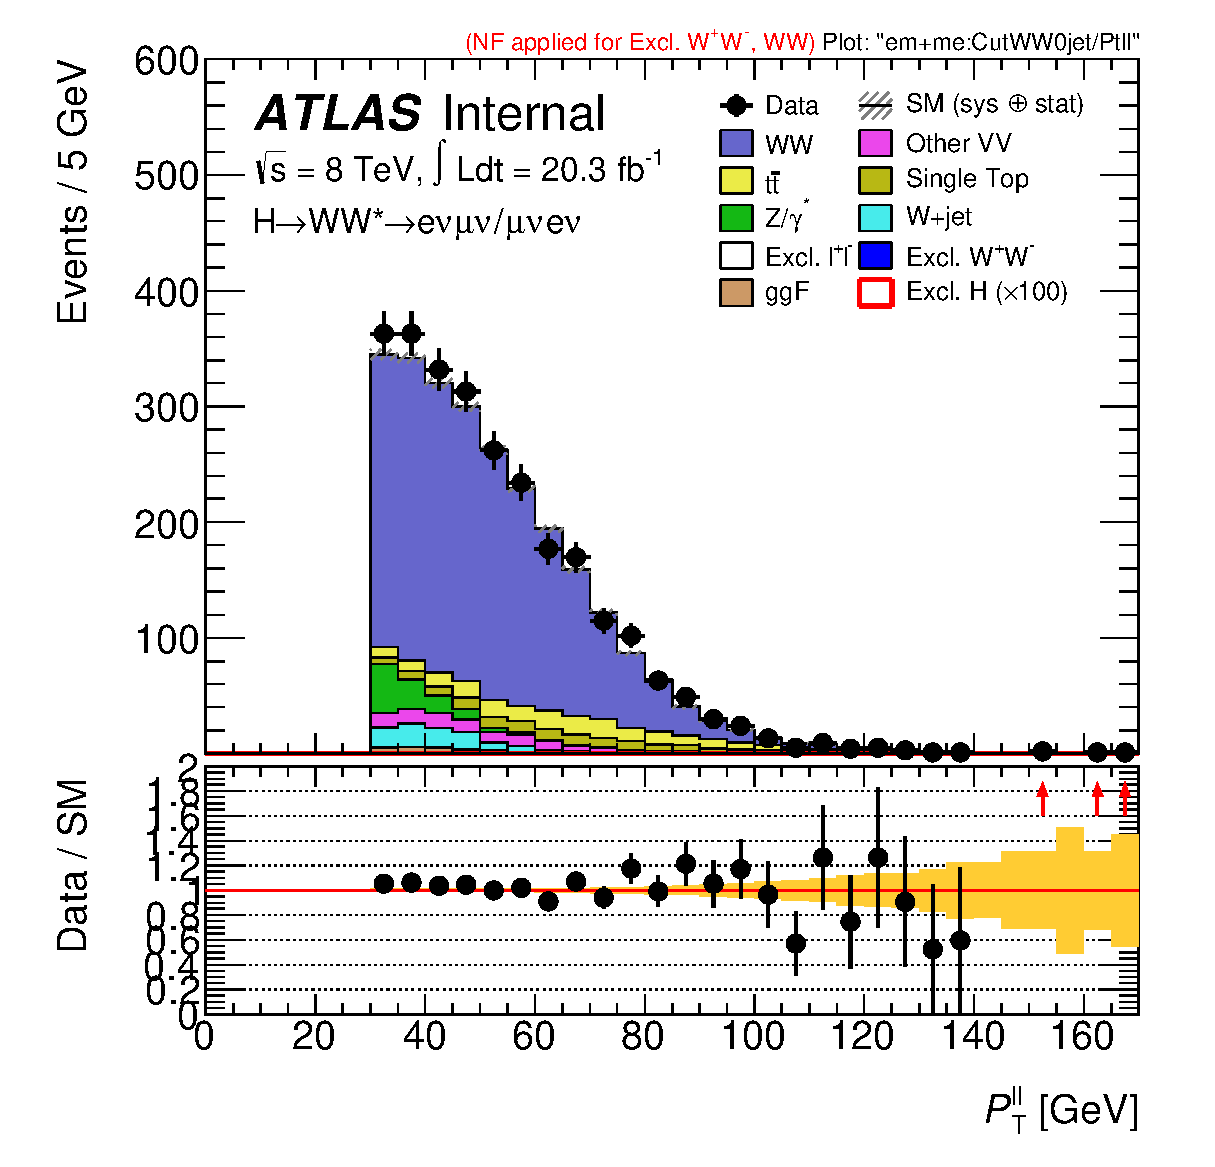
\includegraphics[width=0.5\linewidth]{emme_CutWW0jet_Ptll_mh125_lin.eps}
	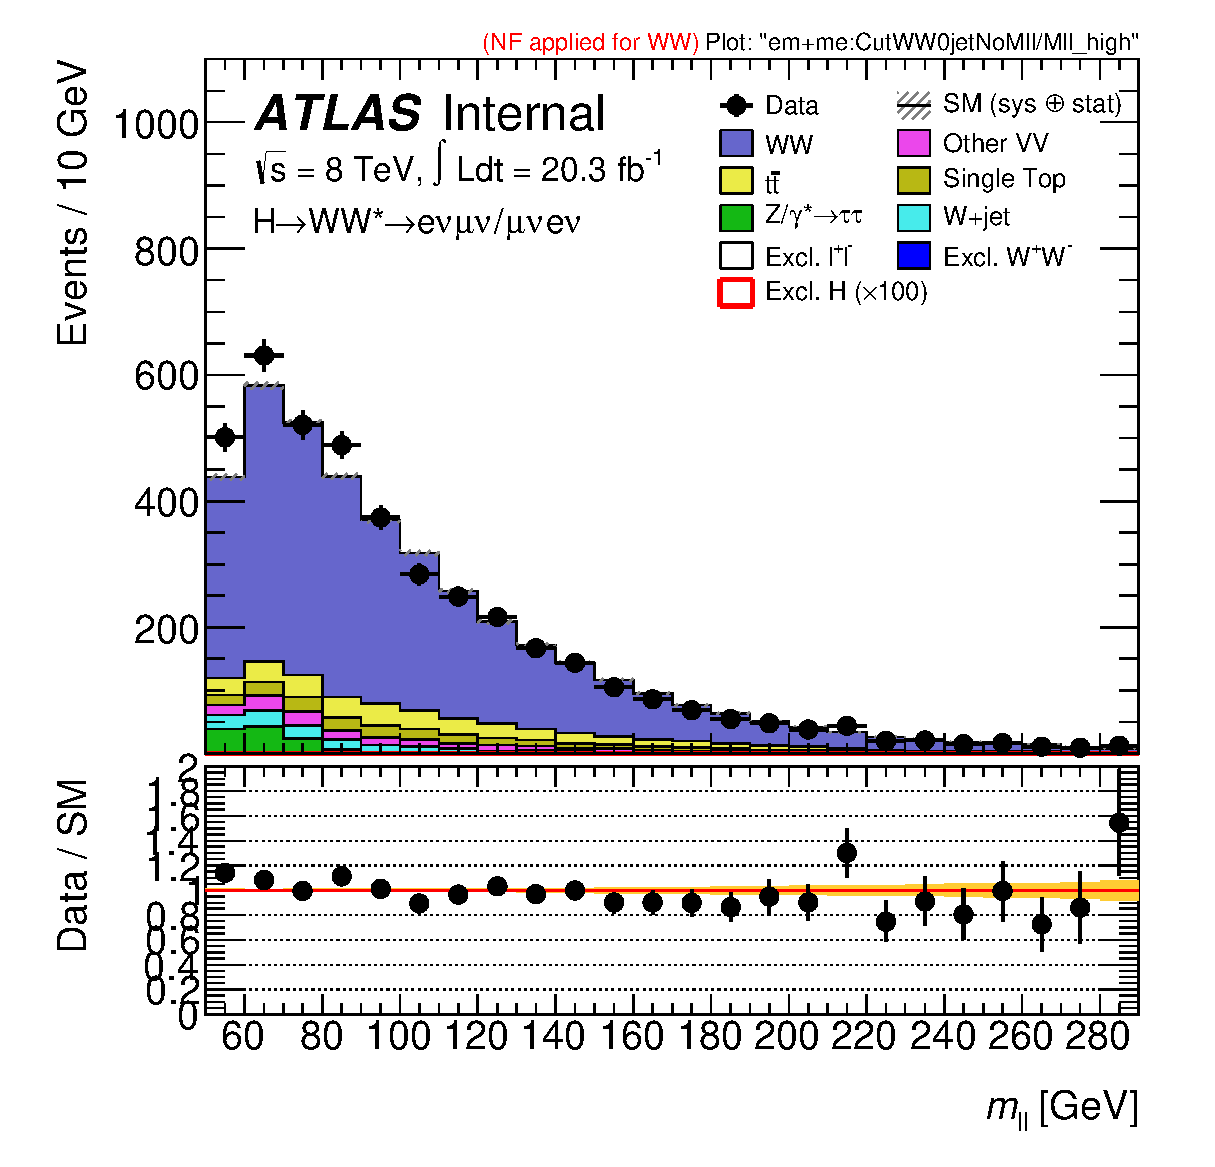
\includegraphics[width=0.5\linewidth]{emme_CutWW0jetNoMll_Mll_high_mh125_lin.eps}\\
	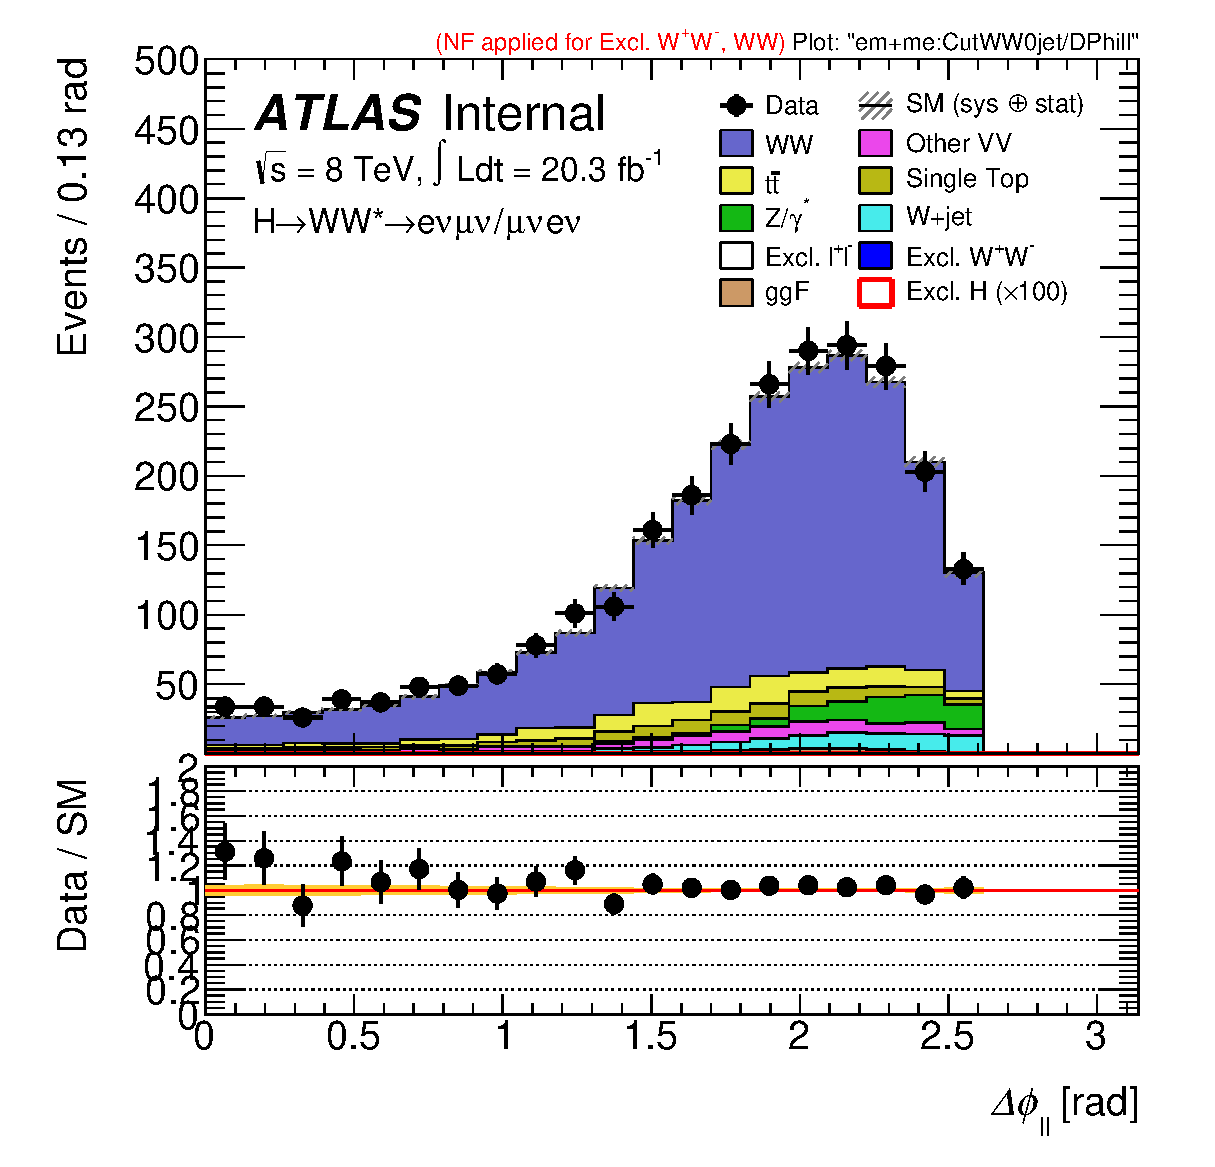
\includegraphics[width=0.5\linewidth]{emme_CutWW0jet_DPhill_mh125_lin.eps}
	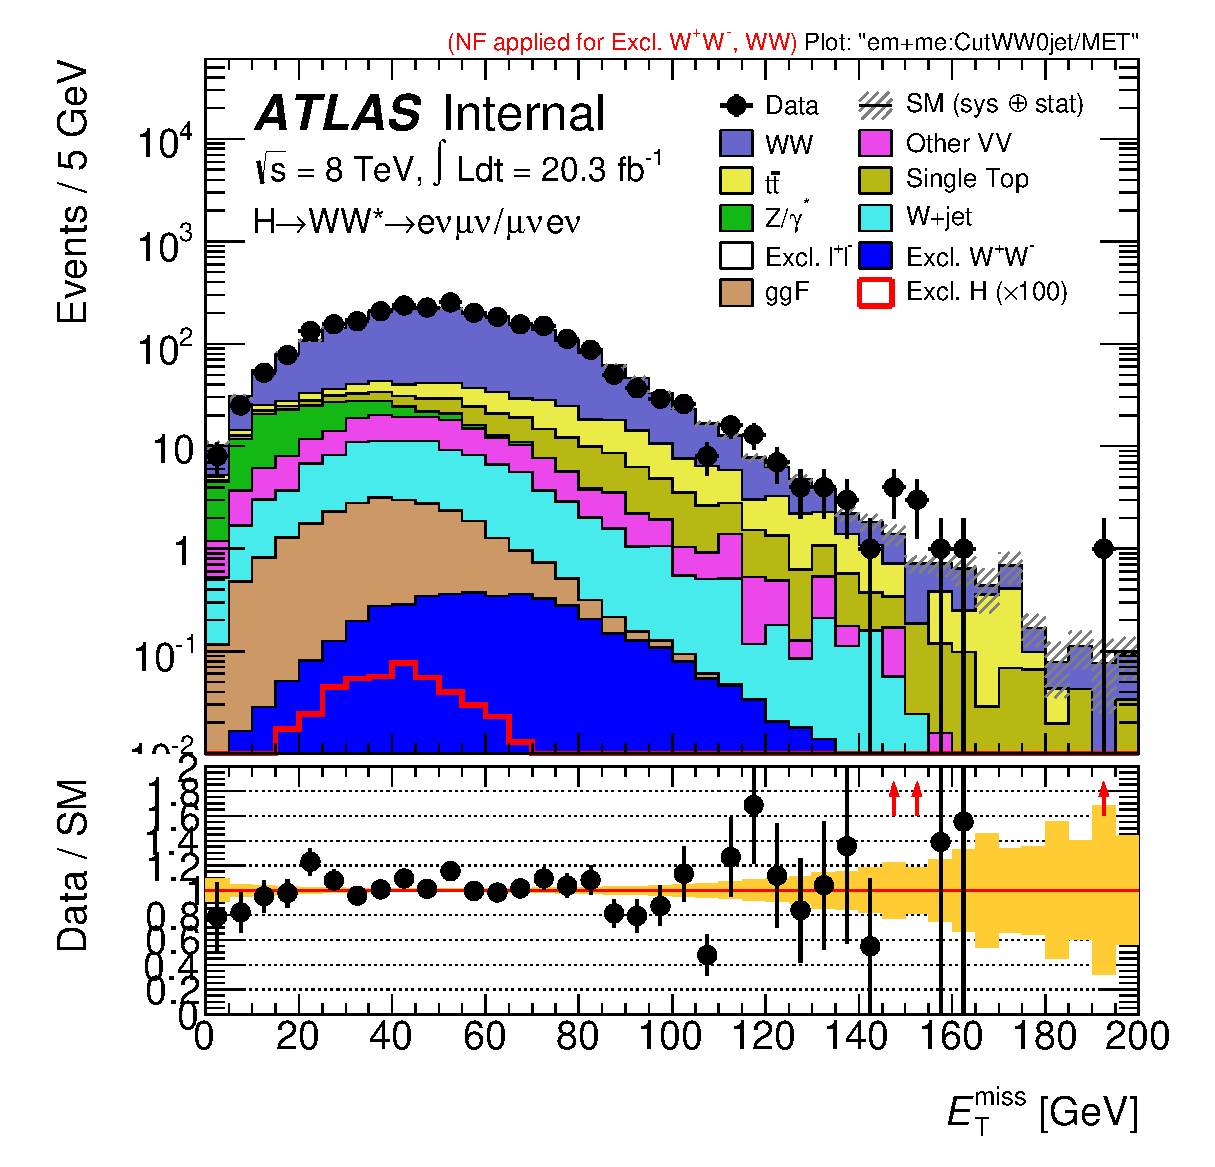
\includegraphics[width=0.5\linewidth]{emme_CutWW0jet_MET_mh125_log.eps}\\
	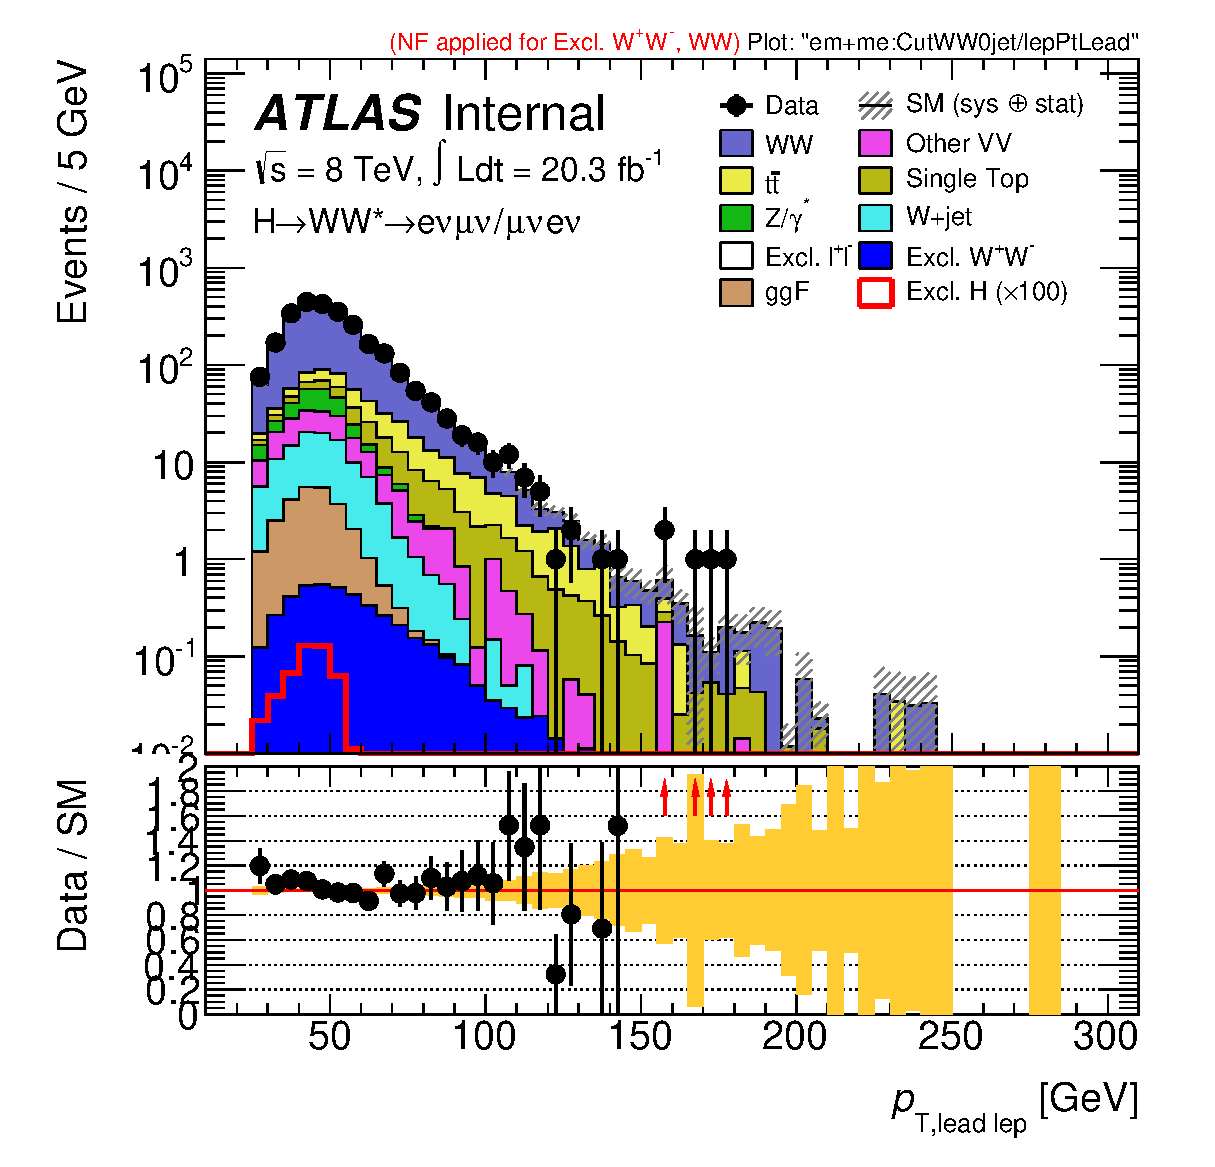
\includegraphics[width=0.5\linewidth]{emme_CutWW0jet_lepPtLead_mh125_log.eps}
	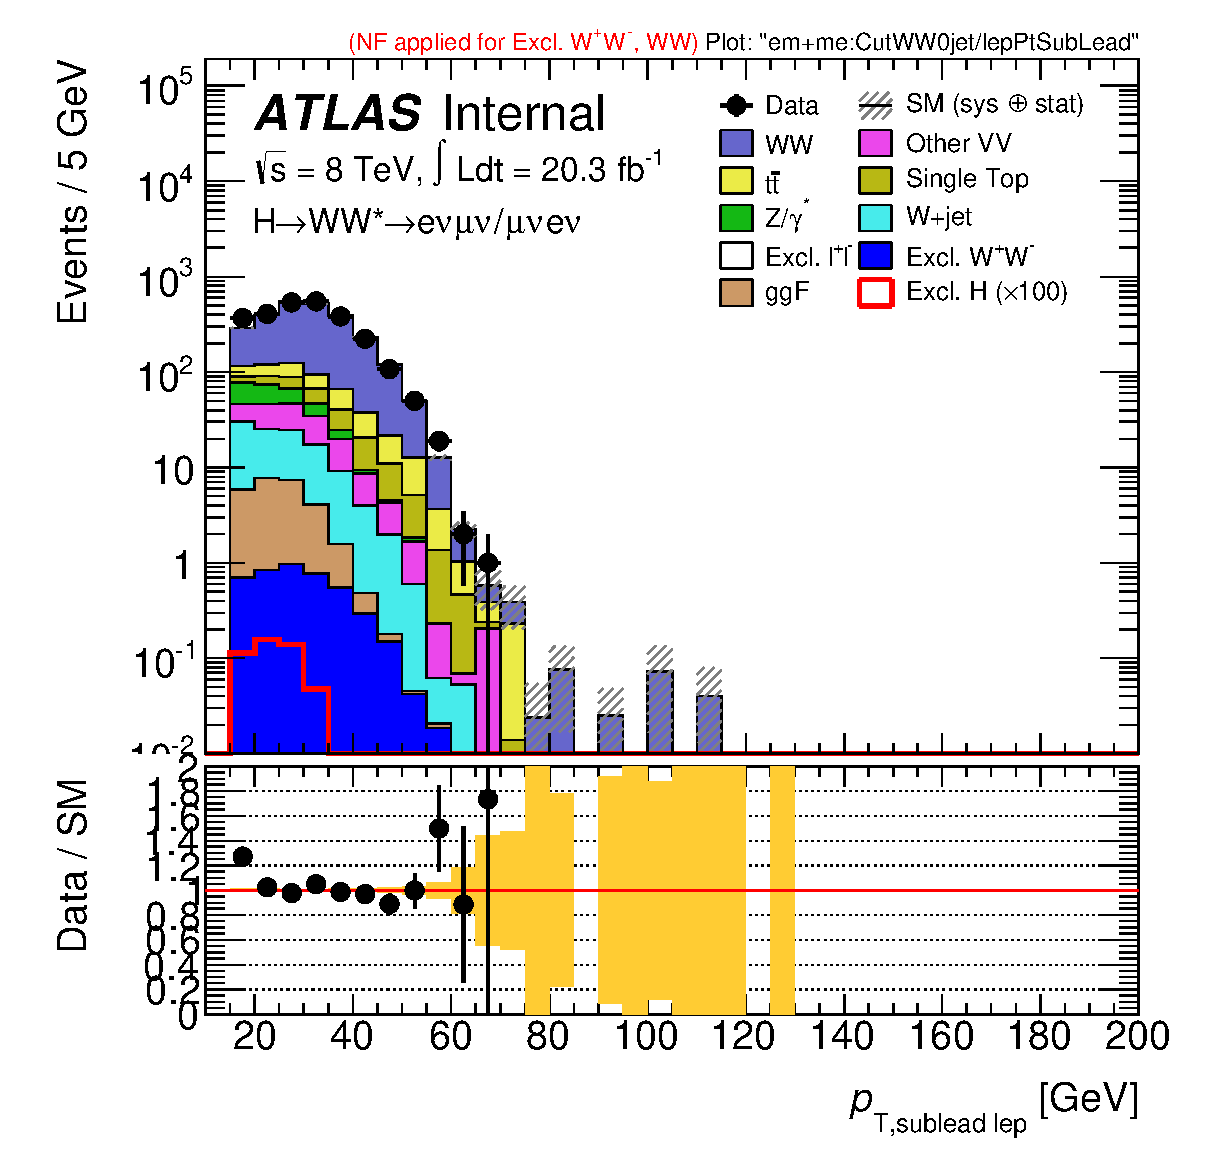
\includegraphics[width=0.5\linewidth]{emme_CutWW0jet_lepPtSubLead_mh125_log.eps}\\
\end{tabular}
\caption{Key kinematic distributions in the WW control region before the exclusivity cut is imposed.}
\label{fig:wwCR}
\end{figure}

\begin{figure}[!h]
\centering
	\includegraphics[width=0.5\linewidth]{emme_CutWW0jet_trkdz0_asymm_mh125_log.eps}
\caption{Exclusivity variable $\Delta z_1$ after an MF has been applied on the inclusive WW process, 
and a flux factor has been applied on the exclusive WW process.}
\label{fig:exclwwCR}
\end{figure}

\begin{table}
\centering
        \resizebox{\textwidth}{!}{
\providecommand{\cutflowTitle}{}
\begin{tabular}{l||rrr|rrr}
Cuts & $WW$ & Excl. $W^{+}W^{-}$ & Other Bkgs & Total Bkg. & Observed & Data/MC \\
\hline\hline
WW CR [$55<m_{\ell\ell}<110$ GeV,$\Delta\phi_{\ell\ell}<2.6$] & 2755.90 $\pm$ 9.99 & 1.48 $\pm$ 0.02 & 9750.32 $\pm$ 153.94 & 12513.27 $\pm$ 154.26 & 12176 & 0.97 $\pm$ 0.01 \\
0 jet & 1946.03 $\pm$ 8.42 & 4.35 $\pm$ 0.05 & 795.62 $\pm$ 133.21 & 2750.17 $\pm$ 133.47 & 2644 & 0.96 $\pm$ 0.05 \\
1 mm Exclusive & 1.21 $\pm$ 0.14 & 2.39 $\pm$ 0.03 & 0.47 $\pm$ 0.32 & 4.07 $\pm$ 0.35 & 9 & 2.21 $\pm$ 0.76 \\
\end{tabular}
}
\caption{Estimated and observed events in the WW CR.}
\label{table:wwCR}
\end{table}

\par The inclusive WW contribution to the signal region turns out to be $0.77\pm0.10$ events.

\subsection{Other Backgrounds}
\par The rest of the backgrounds are estimated using MC, except for the W+jets. Events are selected in data 
that have exactly two leptons, one tightly identified and the other loosely but not tightly identified. These 
events turn out to be 85\% W+jets. All other backgrounds are subtracted from this data sample to obtain a better 
estimation of the W+jets in data. All the backgrounds that use MC are applied appropriate MFs except for exclusive 
dileptons. A flux factor of 2.99 is applied to the exclusive dileptons estimate, which only estimates purely 
elastice processes. A list of all the MC generators used are listed in Table~\ref{table:background}. 
We estimate $0.10\pm0.06$ from all these backgrounds.

%%%%%%%%%%%%%%%%%%%%

%%%%%%%%%%%%%%%%%%%%
%\clearpage
\section{Systematic Uncertainties}
\label{sec:syst}

\par The majority of sources for systematic uncertainties is shared by the search the inclusive ggF 
Higgs through $WW^*$. Additional sources of uncertainties are from the exclusivity cuts. Track impact parameter
measurement and track \pt\ measurement are the major sources of uncertainties
from exclusivity cuts. This area of study is a major work in progress. 

%%%%%%%%%%%%%%%%%%%

\section{Results}
\label{sec:results}

To investigate the sensitivity of this search with the current exclusivity cuts 
we use the transverse mass $m_T$ to perform a fit. Figure~\ref{fig:mT}
shows the $m_T$ distributions for the signal and all the backgrounds.
Z+jets and W+jets are estimated by scaling using exclusivity efficiencies obtained 
from data. The assumption here is that the shape change for these samples due to 
the exclusivity cut is not very significant. An investigation on the validity of this 
assumption is an active area of research. 
 
\begin{figure}[!h]
\centering
\begin{tabular}{c}
	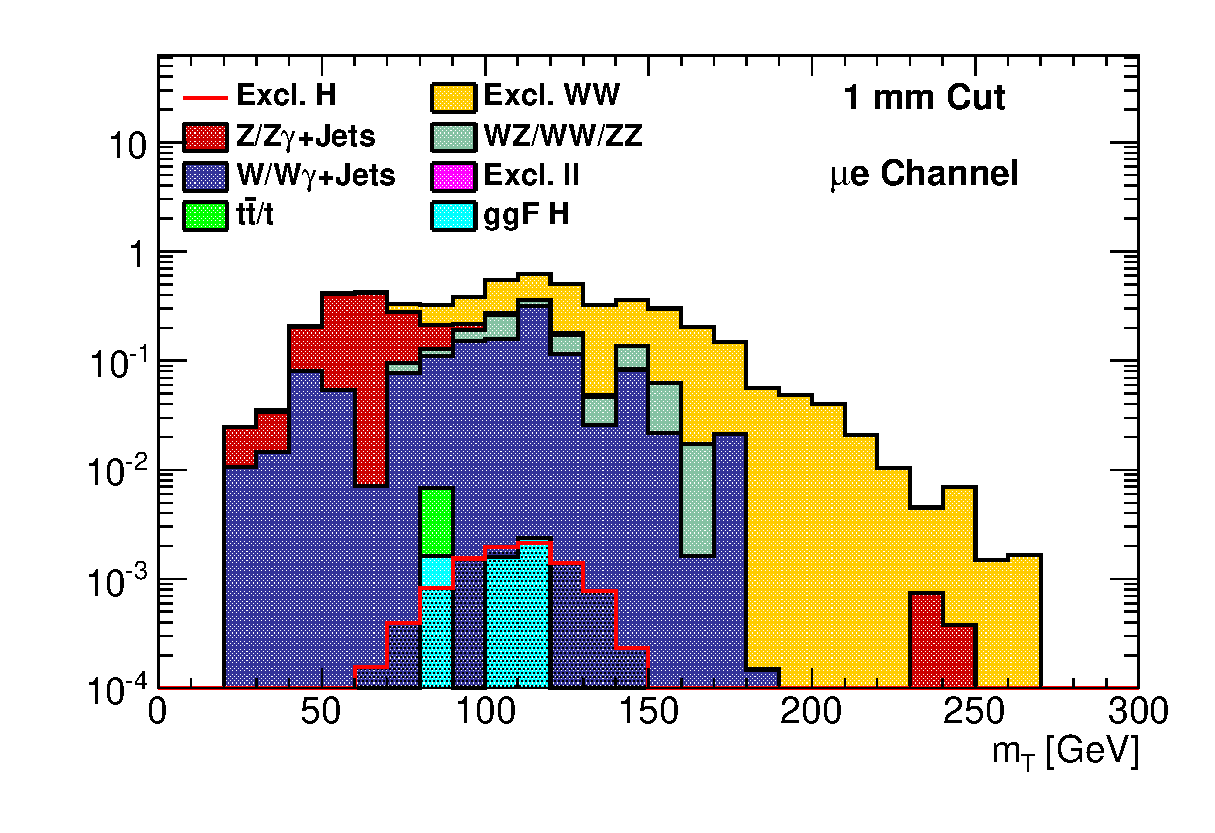
\includegraphics[width=0.5\linewidth]{h_mT_sig_mue.eps}
	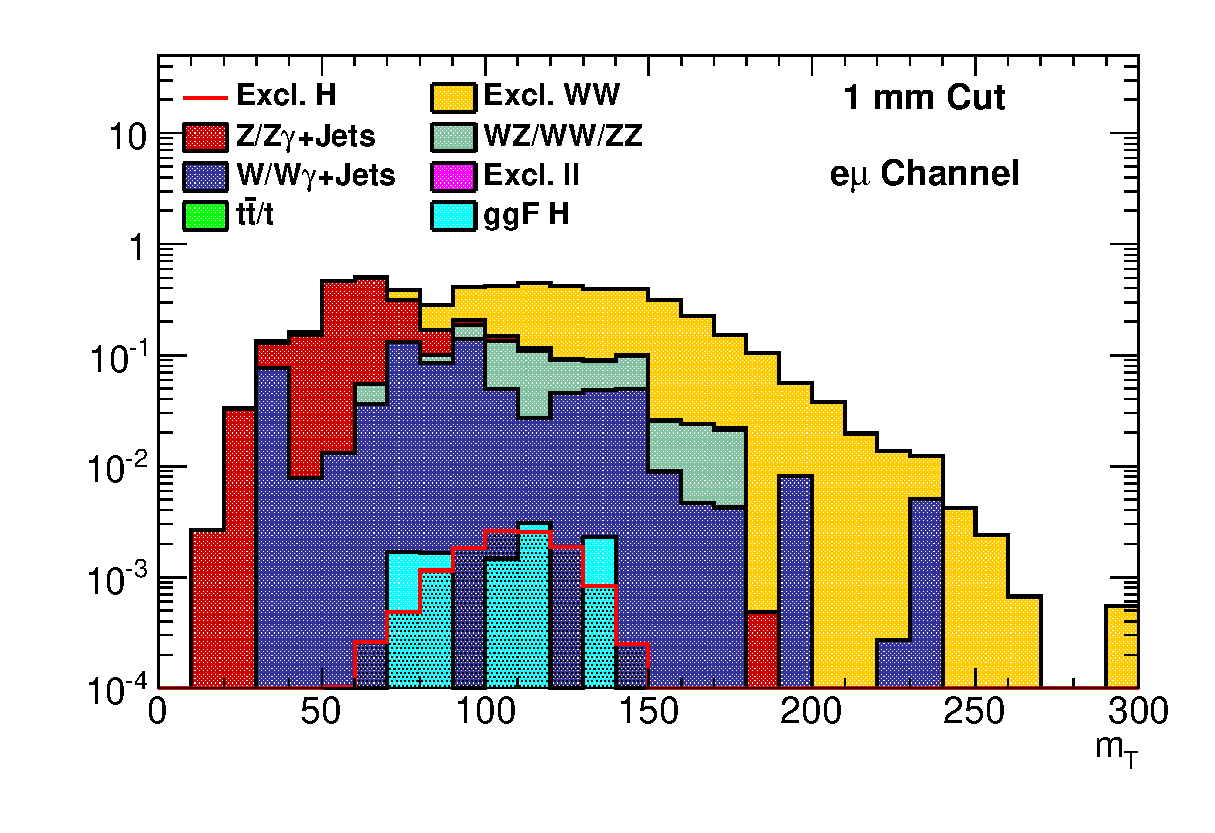
\includegraphics[width=0.5\linewidth]{h_mT_sig_emu.eps}
\end{tabular}
\caption{$m_{T}$ distributions for signal and background. The signal is not part of the stack.}
\label{fig:mT}
\end{figure}

The fit performed in a 1-bin fit for $75<m_T<150\ GeV$. The only systematic uncertainty accounted for 
here is the uncertainty associated with the integrated luminosity. The majority of the uncertainties 
are therefore statistical. Table~\ref{table:limits} shows the limits obtained. 

\begin{table}[!h]
\begin{center}
\begin{tabular}{cc|cccc}
Cut & Limit [pb] & $+1\sigma$ & $+2\sigma$ & $-1\sigma$ & $-2\sigma$ \\
\hline
1 mm & 1.19 & 1.78 & 2.67 & 0.86 & 0.64 \\
\end{tabular}
\end{center}
\caption{Limits set by fitting with $m_T$.}
\label{table:limits}
\end{table}

These limits exclude .... 

%%%%%%%%%%%%%%%%%%%%

\clearpage
\section{Summary}
\label{sec:summary}

\par Studies on the exclusive higgs could provide a very clean channel to further study 
properties of the higgs boson. It is therefore important to quantify the production cross 
section of this process with the current available data that corresponds to LHC's 8 TeV 
collision energy. Previous analyses that studied exclusive processes have exploited the existence 
of rapidity gaps and used reconstructed vertices with their associated tracks to devise 
exclusivity selection criteria. These techniques are not as efficient with pileup that results 
from the 8 TeV collision energy.
\par In this analysis the exclusive Higgs was searched for in the \hwwll\ decay channel. 
Exclusivity selection criteria that are dependent on the two lepton tracks were developed.
These criteria are sensitive to pileup and are expected to become ineffective with high 
pile up in Run II, at 13 TeV collision energy. The major backgrounds to exclusive \hwwll\ are
the inclusive and exclusive WW. All other backgrounds were considered but have very low 
contributions to the signal region. A limit on the total production cross section of 770 fb was 
obtained for the exclusive Higgs. This shows that this analysis is not sensitive to the KMR 
model for the exclusive Higgs, which predicts 3 fb at 8 TeV.
\par Systematic uncertainties are currently being evaluated and the quoted limit is also 
being updated.    

%%%%%%%%%%%%%%%%%%%%

%%%%%%%%%%%%%%%%%%%%%%%%%%%%%%%%%%%%%%%%%%%%%%%%%%%%%%%%%%%%%%%%%%%%%%%%%%%%%%%
% Bibliography
%%%%%%%%%%%%%%%%%%%%%%%%%%%%%%%%%%%%%%%%%%%%%%%%%%%%%%%%%%%%%%%%%%%%%%%%%%%%%%
\clearpage
\bibliographystyle{atlasnote}
\bibliography{notex}

\end{document}
